\documentclass[paper = a4, fleqn, abstract=on, twoside]{scrreprt}
% escapeinside
%\usepackage[gray]{xcolor}
\usepackage[T1]{fontenc}        % T1-Fonts
\usepackage[utf8]{inputenc}     % Enkodierung
\usepackage[english]{babel}
\usepackage{amsmath}
\usepackage{amssymb}
\usepackage{proof} % http://www.logicmatters.net/resources/ndexamples/proofsty.html
\usepackage{bussproofs}
\usepackage{hyperref}
\usepackage{subcaption}
\usepackage{tikz}
\usepackage{natbib}
\usepackage[automark, headsepline]{scrlayer-scrpage}

% Kapitelüberschrift in der Kopfzeile
%\usepackage[automark]{scrpage2} % Schickerer Satzspiegel mit KOMA-Script
%\pagestyle{scrheadings}

% Minted
\usepackage{minted}
\usemintedstyle[haskell]{trac}
\newminted{haskell}{fontsize=\small}
\newminted{coq}{fontsize=\small}

% Für schönere Tabellen (optional)
% \usepackage{booktabs}           % Netteres Tabellenlayout
% \usepackage{multicol}           % Mehrspaltige Bereiche
% \usepackage{tabularx}           % Tabellen mit fester Breite

% Für Listings
% \usepackage{listings}

% Eine kleine Hilfe für offene Lücken
\newcommand{\todo}[1]{\marginpar{\textbf{TODO:} #1}}
\newcommand{\coqinline}[1]{\mintinline{coq}{#1}}

\begin{document}

\pagenumbering{roman} % römische Seitenzahlen

\begin{titlepage}
	\vspace*{3cm}
	\centering
	{\huge\bfseries Formalizing inference systems in Coq by means of type systems for Curry\par}
	\vspace{1cm}
	\textbf{Niels Bunkenburg} \par 
	\vspace{6cm}
	\textbf{Bachelor's Thesis} \par
	Programming Languages and Compiler Construction \par
	Department of Computer Science \par
	Christian-Albrechts-University of Kiel
	\vfill
	Advised by\par
	Prof. Dr. Michael Hanus \par
	M. Sc. Sandra Dylus
	\vfill
	% Randloses Drucken nicht möglich...
	%\tikz[remember picture,overlay] \node[opacity=0.3,inner sep=0pt] at (9.5,-1.5){
\includegraphics{images/cau-siegel-1400.png}};
	{\large \today\par}
\end{titlepage}

\begin{abstract}
	content...
\end{abstract}

% Verzeichnisse
\renewcommand{\contentsname}{Contents}
\tableofcontents   % Inhaltsverzeichnis
\listoffigures     % Abbildungsverzeichnis
% \listoftables      % Tabellenverzeichnis
% \lstlistoflistings % Abbildungsverzeichnis

\newpage               % Expliziter Umbruch für Seitenzahlen
\pagenumbering{arabic} % arabische Seitenzahlen

% Inhalt

% Entweder ausgegliedert in Dateien:
%   \include{chapter/introduction}
%   \include{chapter/fundamentals}
% oder direkt:

\chapter{Introduction}
Does a program behave as intended? This question is a fundamental part of the formal verification of software. One aspect of formal verification is deductive verification, that is, formally representing and proving properties about programs.\citep{filliatre2011deductive} Interactive theorem provers, such as Coq, offer a specification language to represent programs and verification logic to argue about properties of the program. Figure \ref{coqscreen} shows CoqIde, a graphical interface for Coq. The specification is written on the left-hand side; the right-hand side contains an overview of the remaining goals in a proof.
\begin{figure}[H]
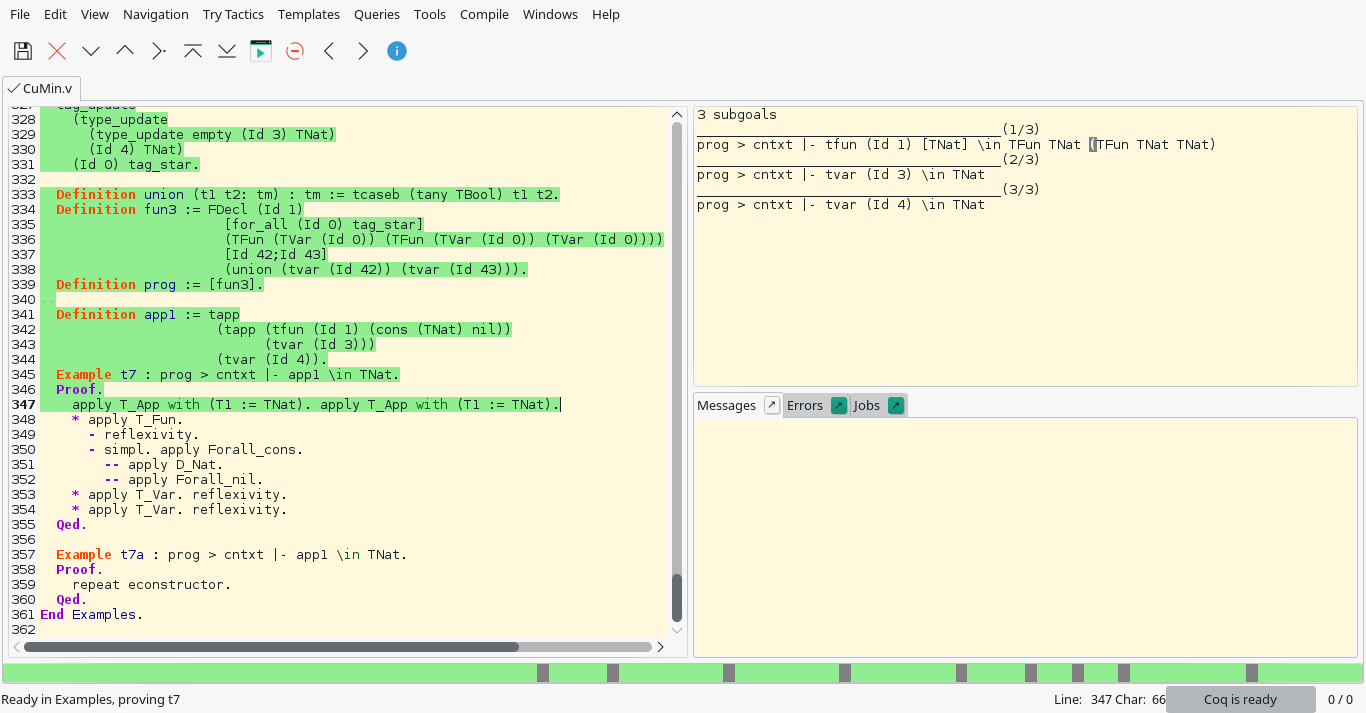
\includegraphics[width=\linewidth]{images/coq.png}
\caption{CoqIde, a graphical interface for Coq}
\label{coqscreen}
\end{figure}\noindent 
In the following chapters, we will use Coq to formalize inference systems, particularly type systems for the functional logic programming language Curry. Type systems are an important concept of strongly typed languages like Curry. Every function and expression has a specific type that, if not explicitly stated, is inferred and checked by the compiler.
The process of typing expressions follows a set of inference rules that define conditions, which need to be met in order for an expression to be of a certain type.\\
\par \noindent
The goal of this thesis is to find an appropriate representation of Curry code in Coq and to implement the inference rules of the type system in order to verify properties of Curry code and to provide a basis for the formalization of further aspects of Curry.\\
\par \noindent
This thesis is structured the following way: We begin with the preliminaries in \autoref{preliminiaries}, which includes a basic introduction to Curry and Coq. The last section of this chapter gives a theoretical overview of the approach used in the following chapters.\\
\par \noindent
Both chapters \ref{cumin} and \ref{flatcurry} are structured similarly: \autoref{cumin} features the language CuMin, a minimal representation of Curry mostly used in theoretical contexts, while \autoref{flatcurry} focuses on FlatCurry, a more practical representation that is used as an intermediary language for some Curry compilers.
The common approach in these chapters includes discussing and implementing the syntax of both languages and the type system. Chapter \ref{cumin} ends with a few examples and a section about automated proofs, while \autoref{flatcurry} is concluded with a program that transforms Curry programs into a Coq-compatible form.\\
\par \noindent
The last chapter presents the results and possible expansions thereof, as well as related work. 
\chapter{Preliminaries}
\label{preliminiaries}
This chapter introduces the two main programming languages used in this thesis: Coq and Curry. The introduction of Coq is based on \textit{Software Foundations} by \citet{Pierce:SF} and gives an overview of modeling and proving in Coq. In case of Curry, we focus on the extended features compared to Haskell.
In the last section the approach and languages used in the following chapters are presented.
\section{Coq}
The formalization of Curry programs requires a language that allows us to express the code itself and propositions we intend to prove. Coq is an interactive proof management system created by \cite{CoqManualV8} that meets these requirements with its functional modeling language and integrated verification logic.
\par
We already saw CoqIde in \autoref{coqscreen}, but this is not the only Coq front-end. There is also the Emacs package \textit{Proof General}\footnote{https://proofgeneral.github.io/} that integrates multiple interactive theorem provers like Coq into the text editor.
\par 
Regardless of the interface chosen, the structure is similar to the following: the left-hand side contains the code, while the right-hand side shows information about proofs and error messages. Definitions in Coq are always completed by a dot that marks a segment. Depending on the front-end, there may be buttons or shortcuts to load one segment at a time, multiple segments or the whole file. A loaded segment is usually highlighted green, which means that the definition contains no errors.
\par
Because of this approach, definitions that reference other definitions need to be in the correct order, that is, a function or data structure needs to be defined before expressions can use it. 
\subsection{Data types and functions}
Coq's predefined definitions, contrary to e.g. Haskell's Prelude, are very limited. Nevertheless, being a functional language, there is a powerful mechanism for defining new data types. A definition of polymorphic lists could look like this:
\begin{coqcode}
Inductive list (X:Type) : Type :=
  | nil  : list X
  | cons : X -> list X -> list X.
\end{coqcode}
We defined a type named \coqinline{list} with two constructors: the constant \coqinline{nil}, which represents an empty list, and a binary constructor \coqinline{cons} that takes an element and a list of the same type as arguments. In fact, \coqinline{nil} and \coqinline{cons} have one additional argument, a type \coqinline{X}. This is required, because we want polymorphic lists -- but we do not want to explicitly state the type. Fortunately, Coq allows us to declare type arguments as implicit by enclosing them in curly brackets:
\begin{coqcode}
Check (cons nat 8 (nil nat)). (*cons nat 8 (nil nat) : list nat*)
Arguments nil {X}.
Arguments cons {X} _ _.
\end{coqcode}
Coq's type inference system infers the type of a list automatically now if possible. In some cases this does not work, because there is not enough information about the implicit types present. 
\begin{coqcode}
Fail Definition double_cons x y z := (cons x (cons y z)).
Definition double_cons {A} x y z := (@cons A x (@cons A y z)).
\end{coqcode}
The first definition does not work, as indicated by \coqinline{Fail}\footnote{\coqinline{Fail} checks if an expression does indeed cause an error and allows further processing of the file.}, because Coq cannot infer the implicit type variable of \coqinline{double_cons}, since \coqinline{cons} does not have an explicit type either. By prefixing at least one \coqinline{cons} with \coqinline{@}, we can tell Coq to accept explicit expressions for all implicit arguments. This allows us to pass the type of \coqinline{cons} on to \coqinline{double_cons}, again as an implicit argument.
\begin{coqcode}
Check double_cons 2 4 []. (* : list nat *)
Fail Check (cons 2 (cons nil nil)). 
(* Error: The term "cons nil nil" has type "list (list ?X0)"
while it is expected to have type "list nat". *)
\end{coqcode}
Based on this we can write a function that determines if a list is empty:
\begin{coqcode}
Definition isEmpty {X : Type} (l : list X) : bool := 
  match l with
  | nil      => true
  | cons _ _ => false
  end.
\end{coqcode}
Function definitions begin with the keyword \coqinline{Definition}. \coqinline{isEmpty} takes an (implicit) type and a list and returns a boolean value.
To distinguish empty from non-empty lists, pattern matching can be used on $n$ arguments by writing \coqinline{match} $x_{0},...,x_{n-1}$ \coqinline{with} | $p_{0} \rightarrow e_{0}$ | ... | $p_{m-1} \rightarrow e_{m-1}$ for $m$ pattern $p$, consisting of a sub-pattern for every $x_{i}$ and expressions $e_{i}$.

The definition of recursive functions requires that the function is called with a smaller structure than before in each iteration, which ensures that the function eventually terminates. A recursive function is indicated by using \coqinline{Fixpoint} instead of \coqinline{Definition}.
\begin{coqcode}
Fixpoint app {X : Type} (l1 l2 : list X) : (list X) :=
  match l1 with
  | nil => l2
  | cons h t => cons h (app t l2)
  end.
\end{coqcode}
In this case $l_{1}$ gets shorter with every iteration and thus the function terminates after a finite number of recursions. 

Coq allows us to define notations for functions and constructors by using the keyword \coqinline{Notation}, followed by the desired syntax and the expression. 
\begin{coqcode}
Notation "x :: y" := (cons x y) (at level 60, right associativity).
Notation "[ ]" := nil.
Notation "[ x ; .. ; y ]" := (cons x .. (cons y []) ..).
Notation "x ++ y" := (app x y) (at level 60, right associativity).
\end{coqcode}

\subsection{Propositions and proofs}
Every claim that we state or prove has the type \coqinline{Prop}. Propositions can be any statement, regardless of its truth. A few examples:
\begin{coqcode}
Check 1 + 1 = 2. (* : Prop *)
Check forall (X : Type) (l : list X), l ++ [] = l. (* : Prop *)
Check forall (n : nat), n > 0 -> n * n > 0. (* : Prop *)
Check (fun n => n <> 2). (* : nat -> Prop*)
\end{coqcode}
The first proposition is a simple equation, while the second one contains an universal quantifier. This allows us to state propositions about every type of list, or, as shown in the third example, about every natural number greater than zero. Combined with implications we can premise specific properties that limit the set of elements the proposition applies to. The last example contains an anonymous function, which is used by stating the functions' arguments and an expression.
\par
Now how do we prove these propositions? Proving an equation requires to show that both sides are equal, usually by simplifying one side until it looks exactly like the other. Coq allows us to do this by using tactics, which can perform a multitude of different operations.
\begin{coqcode}
Example e1 : 1+1=2.
Proof. simpl. reflexivity. Qed. 
\end{coqcode} 
\todo{Highlighting für Proof und Qed}
After naming the proposition as an example, theorem or lemma it appears in the interactive subgoal list that Coq provides. The \coqinline{simpl} tactic performs basic simplification like adding two numbers in this case. The updated subgoal is now \coqinline{2=2}, which is obviously true. By using the \coqinline{reflexivity} tactic we tell Coq to check both sides for equality, which succeeds and clears the subgoal list, followed by \coqinline{Qed} to complete the proof.
\begin{coqcode}
Example e2 : forall (X : Type) (l : list X), [] ++ l = l.
Proof. intros X l. reflexivity. Qed.
\end{coqcode}
Universal quantifiers allow us to introduce variables, the corresponding tactic is called \coqinline{intros}. The new context contains a type \coqinline{X} and a list \coqinline{l}, with the remaining subgoal \coqinline{[ ] ++ l = l}. Because we defined \coqinline{app} to return the second argument if the first one is an empty list, \coqinline{reflexivity} directly proves our goal. \coqinline{reflexivity} is not useful for obvious equations only, it also simplifies and unfolds definitions until the flat terms match each other if possible.
\par
To prove that the proposition \coqinline{l ++ [] = l} holds, we need more advanced tactics, because we cannot just apply the definition. \coqinline{app} works by iterating through the first list, but we need to prove the proposition for every list, regardless of its length. One possibility to solve this problem is by using structural induction.
\begin{coqcode}
Example e3 : forall (X : Type) (l : list X), l ++ [] = l.
Proof. intros X. induction l as [|l ls IH].
  reflexivity.
  simpl. rewrite IH. reflexivity.
Qed.
\end{coqcode}
The proof begins by introducing type \coqinline{X}, followed by the \coqinline{induction} tactic applied to \coqinline{l}. Coq names newly introduced variables by itself, which can be done manually by adding \coqinline{as [c1|...|cn]} to the tactic. Each $c_{i}$ represents a sequence of variable names, which will be used when introducing variables in the corresponding case. Cases are ordered as listed in the \coqinline{Definition}.
\par
Now we need to prove two cases: the empty list and a cons construct. The first case does not require any new variable names, therefore the first section in the squared brackets is empty. It is easily solved by applying \coqinline{reflexivity}, because of the definition of \coqinline{app}.
The second case requires variables for the list's head and tail, which we call \coqinline{l} and \coqinline{ls} respectively. The variable name \coqinline{IH} identifies the induction hypothesis \coqinline{ls ++ [ ] = ls}, which Coq generates automatically. The goal changes as following:
\begin{coqcode}
(l :: ls) ++ [ ] = l :: ls
 l :: ls  ++ [ ] = l :: ls (* simpl *)
 l :: ls         = l :: ls (* rewrite with IH *)
\end{coqcode}
The tactic \coqinline{rewrite} changes the current goal by replacing every occurrence of the left side of the provided equation with the right side. Both sides are equal now and therefore \coqinline{reflexivity} proves the last case.
\par 
Example \coqinline{e4} is different from the other examples, in the sense that one cannot prove a function by itself and that only supplying an argument returns a verifiable inequality. 
\begin{coqcode}
Example e4 : (fun n => n <> 2) 1.
Proof.
  simpl.       (* 1 <> 2 *)
  unfold not.  (* 1 = 2 -> False *)
  intros H.    (* H : 1 = 2, False *)
  inversion H. (* No more subgoals. *)
Qed.
\end{coqcode}
This proof is not as straight forward as the other ones, mainly because of the inequality, which is a notation\footnote{It is often useful to be able to look up notations, \coqinline{Locate "<>"} returns the term associated with \coqinline{<>}.} for \coqinline{not (x = y)}. Because \coqinline{not} is the outermost term, we need to eliminate it first by applying \coqinline{unfold}. This replaces \coqinline{not} with its definition \coqinline{fun A : Prop => A -> False}, where \coqinline{False} is the unprovable proposition. Why does this work?
Assuming that a proposition \coqinline{P} is true, \coqinline{not P} means that \coqinline{P} implies \coqinline{False}, which is false, because something true cannot imply something false. On the other hand, if \coqinline{P} is false, then \coqinline{False -> False} is true because anything follows from falsehood, as stated by the principle of explosion. \todo{verweis?}
\par
The current goal \coqinline{4 = 8 -> False} is further simplified by introducing \coqinline{4 = 8} as an hypothesis \coqinline{H}, leaving \coqinline{False} as the remaining goal. Intuitively we know that \coqinline{H} is false, but Coq needs a justification for this claim.
Conveniently the tactic \coqinline{inversion} solves this problem easily by applying two core principles of inductively defined data types:
\begin{itemize}
	\item Injectivity: \coqinline{C n = C m} implies that n and m are equal for a constructor \coqinline{C}.
	\item Disjoint constructors: Values created by different constructors cannot be equal.
\end{itemize}
By applying \coqinline{inversion} to the hypothesis \coqinline{2 = 1} we tell Coq to add all inferable equations as additional hypotheses. In this case we start with \coqinline{2 = 1} or the Peano number representation \coqinline{S(S(O)) = S(0)}. Injectivity implies that if the previous equation was true, \coqinline{S(O) = O} must also be true. This is obviously false, since it would allow two different representations of nil. Hence, the application of \coqinline{inversion} to \coqinline{2 = 1} infers the current goal \coqinline{False}, which concludes the proof.

Besides directly supplying arguments to functions that return propositions, there are other interesting applications for them, that we will discuss in the next section.

\subsection{Higher-order constructs}
Functions can be passed as arguments to other functions or returned as a result, they are first-class citizens in Coq. This allows us create higher-order functions, such as \coqinline{map} or \coqinline{fold}.
\todo{minted bug?}
\begin{coqcode}
Fixpoint map {X Y : Type} (f : X -> Y) (l : list X) : (list Y) :=
  match l with
  | []     => []
  | h :: t => (f h) :: (map f t)
  end.
\end{coqcode}
Function types are represented by combining two or more type variables with an arrow. Coq does not only allow higher-order functions but also higher-order propositions. A predefined example is \coqinline{Forall}, which features a \coqinline{A -> Prop} construct from the last section.
\begin{coqcode}
Forall : forall A : Type, (A -> Prop) -> list A -> Prop
\end{coqcode}
\coqinline{Forall} takes a \textit{property} of \coqinline{A}, which returns a \coqinline{Prop} for any given \coqinline{A}, plus a list of \coqinline{A} and returns a proposition. It works by applying the property to every element of the given list and can be proven by showing that all elements satisfy the property.
\begin{coqcode}
Example e5 : Forall (fun n => n <> 8) [2;4].
Proof.
apply Forall_cons. intros H. inversion H.
(* Forall (fun n : nat => n <> 8) [4] *)
apply Forall_cons. intros H. inversion H.
(* Forall (fun n : nat => n <> 8) [ ] *)
apply Forall_nil.
Qed.
\end{coqcode}
\coqinline{Forall} is an inductively defined proposition, which requires rules to be applied in order to prove a certain goal. This will be further explained in the next section, for now it sufficient to know that \coqinline{Forall} can be proven by applying the rules \coqinline{Forall_cons} and \coqinline{Forall_nil}, depending on the remaining list. Because we begin with a non-empty list, we have to apply \coqinline{Forall_cons}. The goal changes to \coqinline{2 <> 8}, the head of the list applied to the property. We have already proven this type of inequality before, \coqinline{inversion} is actually able to do most of the work we did manually by itself. Next the same procedure needs to be done for the list's tail \coqinline{[4]}, which works exactly the same as before. To conclude the proof, we need to show that the property is satisfied by the empty list. \coqinline{Forall_nil} covers this case, which is trivially fulfilled.
\subsection{Inductively defined propositions}
\label{induprop}
Properties of a data type can be written in multiple ways, two of which we already discussed: Boolean equations of the form \coqinline{b x = true} and functions that return propositions. For example the function \coqinline{InB} returns \coqinline{true} if a \coqinline{nat} is contained in a list, the boolean function could look like this:
\begin{coqcode}
Fixpoint InB (x : nat) (l : list nat) : bool :=
match l with
| [] => false
| x' :: l' => if (beq_nat x x') then true else InB x l'
end.
Example e5 : InB 42 [1;2;42] = true.
Proof. reflexivity. Qed.
\end{coqcode}
Because \coqinline{InB} returns a boolean value, we have to check for equality with \coqinline{true} in order to get a provable proposition. The proof is fairly simple, \coqinline{reflexivity} evaluates the expression and checks the equation, nothing more needs to be done.
\par 
Properties are another approach that works equally well. This definition connects multiple equations by disjunction, noted as \coqinline{\/}. The resulting proposition needs to contain a least one true equation to become true itself.
\begin{coqcode}
Fixpoint In (x : nat) (l : list nat) : Prop :=
match l with
| [] => False
| x' :: l' => x' = x \/ In x l'
end.
Example e6 : In 42 [1;2;42].
Proof. 
  simpl. (* 1 = 42 \/ 2 = 42 \/ 42 = 42 \/ False *)
  right.           (* 2 = 42 \/ 42 = 42 \/ False *)
  right.                     (* 42 = 42 \/ False *)
  left.                      (* 42 = 42 *)
  reflexivity.
Qed.
\end{coqcode}
Proving the same example as before, we need new tactics to work with logical connectives. By simplifying the original statement we get a disjunction of equations for every element in the list. If we want to show that a disjunction is true, we need to choose a side we believe to be true and prove it. \coqinline{left} and \coqinline{right} keep only the respective side as the current goal, discarding the other one. A similar tactic exists for the logical conjunction \coqinline{/\ }, with the difference that \coqinline{split} keeps both sides as subgoals, since a conjunction is only true if both sides are true.
\par
The last option to describe this property is by using inductively defined propositions. As already mentioned before, inductively defined propositions consist of rules that describe how an argument can satisfy the proposition.
\label{In}
\begin{coqcode}
Inductive InInd : nat -> list nat -> Prop :=
| Head : forall n l, InInd n (n :: l)
| Tail : forall n l, InInd n (tl l) -> InInd n l.
\end{coqcode} 
Rule one states that the list's head is an element of the list. Additionally, if an element is contained in a list, it is also an element of the the same list, prefixed by another element, as described in the second rule. This definition can be transferred to Coq:
\begin{coqcode}
Example e7 : InInd 42 [2;42].
Proof. 
  apply Tail.  (* InInd 42 (tl [2; 42]) *)
  simpl.       (* InInd 42 [42] *)
  apply Head.
Qed.           
\end{coqcode}
The interesting part about this proof is the deductive approach. Previously we started with a proposition and constructed evidence of its truth. In this case we use \coqinline{InInd}'s rules "backwards": Because we want to show that \coqinline{42} is an element of \coqinline{[2;42]]}, we need to argue that it is contained within the list's tail. Since it is the head of \coqinline{[42]}, we can then apply \coqinline{Head} and conclude that the previous statement must also be true, because we required \coqinline{42} to be contained in the list's tail, which is true.
\par
Inductively defined propositions will play an important role in the following chapters, hence some more examples:
\begin{coqcode}
Inductive Forall (A : Type) (P : A -> Prop) : list A -> Prop :=
| Forall_nil : Forall P [ ]
| Forall_cons : forall (x : A) (l : list A), P x -> Forall P l -> Forall P (x :: l)
\end{coqcode}
We already used \coqinline{Forall} in the previous section without knowing the exact definition, the rules are fairly intuitive. According to \coqinline{Forall_nil}, a proposition is always true for the empty list. If the list is non-empty, the first element and the list's tail have to satisfy the proposition, as stated in \coqinline{Forall_cons}, in order for the whole list to satisfy the property. This pattern can be expanded to more complex inductive propositions, \coqinline{Forall2} takes a binary property plus two lists and checks if $P ~ a_{i} ~ b_{i}$ holds for every \coqinline{i < length l}.
\begin{coqcode}
Forall2 : forall A B : Type, (A -> B -> Prop) -> list A -> list B -> Prop
\end{coqcode}
\section{Curry}
Curry\citet{report} is a programming language that combines aspects of functional and logical programming. Created by an international initiative, Curry is predominantly aimed at providing a platform for research and teaching.\cite{curryintro} Curry's syntax is similar to Haskell with the addition of nondeterminism, that is, a function can return different values for the same input, and free variables, which allow the systematic search for unknown values.
\par
The similarities to Haskell include the (interactive) compiler KICS2\footnote{https://www-ps.informatik.uni-kiel.de/kics2/} that compiles Curry programs to Haskell code and  an easily searchable\footnote{https://www-ps.informatik.uni-kiel.de/kics2/currygle/}, extensive module system with many predefined data structures and functions. In this short overview we will take a look at some language features that we will work with later, albeit not necessarily in the form of Curry code.\\
\par\noindent
Curry programs have the ending \texttt{.curry} and consist of function and data type declarations. The simplest form of functions, such as \texttt{double x = x + x}, has a name, a possibly empty list of variables and an expression. Although it is not mandatory to explicitly state a function's type, in this case \texttt{double :: Int $\rightarrow$ Int $\rightarrow$ Int}, every function has a type that describes the arguments and the result of evaluating the function. When a function call is evaluated, the left-hand side is replaced with the right-hand side until there is no further evaluation possible, that is, only literal values or data structures remain. The evaluation can result in an infinite loop, for example \texttt{twos = 2 : twos}, or not compute any values. Infinite data structures are processed by computing the value of an expression only if it is actually needed, called \textit{lazy} evaluation. In the example below the function \texttt{take} returns the first $n$ elements of a list. The value of \texttt{twos} is only evaluated by one step when the application of \texttt{take} requires the values of the list's head. Thus, the infinite list can be accessed without computing the whole structure.
\begin{flushleft}
	\begin{minipage}[t]{.3 \linewidth}
		\begin{haskellcode}
take 2 twos
take 2 (2 : twos)
2 : take 1 twos
2 : take 1 (2 : twos)
2 : 2 : take 0 twos
2 : 2 : []
		\end{haskellcode}
	\end{minipage}
	\hfill
	\vrule
	\hspace{.5em}
	\begin{minipage}[t]{.65 \linewidth}
		\begin{haskellcode}
take :: Int -> [a] -> [a]
take n l = if n <= 0 then [] else takep n l
  where takep _ []     = []
        takep m (x:xs) = x : take (m-1) xs
		\end{haskellcode}
	\end{minipage}
\end{flushleft}
\noindent
More advanced functions use several rules and pattern matching to describe different computational paths. By using a pattern in the left-hand side of a rule, it is limited to arguments of a specific form. Thus, functions that process data types with multiple constructors can have a different rule for every constructor. While Haskell allows overlapping patterns, that is, multiple patterns that apply to the same argument, functions remain deterministic because only the first rule that matches the argument is evaluated. Curry does not limit the evaluation -- a function with overlapping patterns can return every possible result an input evaluates to. On the other hand, patterns do not need to be exhaustive, that is, cover every possible input, because a failed computation is a valid result unlike the exception Haskell returns.
\begin{flushleft}
	\begin{minipage}[t]{.3 \linewidth}
		\begin{haskellcode}
failed = head []
eight = failed ? 8
		\end{haskellcode}
	\end{minipage}
	\hfill
	\vrule
	\hspace{.5 em}
	\begin{minipage}[t]{.65 \linewidth}
		\begin{haskellcode}
(?) :: a -> a -> a
x ? _ = x
_ ? y = y
		\end{haskellcode}
	\end{minipage}
\end{flushleft}
\noindent
The function \texttt{head} returns the first element of a list, but in this case the list is empty. Therefore, the computation fails and KICS2 returns an exclamation mark. Nevertheless, it is possible to apply the \texttt{?} operator that represents a non-deterministic choice between the arguments to both the failed computation and the number 8. Since only one argument contains a value, the expression evaluates to 8.
\par
In some situations deterministic programs are inevitable, for example when working with IO actions. While it may not seem import if a function prints an 'a' or 'b' to the terminal, writing a file of non-deterministic size to the hard drive can cause severe problems. Fortunately, Curry enforces determinism when using IO actions. If one needs a more Haskell-esque evaluation of multiple patterns, the \texttt{case} expression applies:
\begin{flushleft}
	\begin{minipage}[t]{.3 \linewidth}
		\begin{haskellcode}
maybeNot True  = False
maybeNot True  = True
maybeNot False = True
maybeNot False = False
		\end{haskellcode}
	\end{minipage}
	\hfill
	\vrule
	\hspace{.5 em}
	\begin{minipage}[t]{.25 \linewidth}
		\begin{haskellcode}
notCase b =
  case b of
    True  -> False
    True  -> True
    False -> True
    False -> False
		\end{haskellcode}
	\end{minipage}
	\hfill
	\vrule
	\hspace{.5 em}
	\begin{minipage}[t]{.35 \linewidth}
		\begin{haskellcode}
maybeNotCase b =
  case b of
    True  -> False ? True 
    False -> True  ? False
		\end{haskellcode}
	\end{minipage}
\end{flushleft}
Pattern matching in a function can be transformed to a corresponding case expression by replacing the pattern with a variable and creating a branch for every rule. The difference is that case expressions evaluate only the first matching branch. Thus, the second and fourth branch of \texttt{caseNot} are not reachable and the function is deterministic. If nondeterminism is needed in a \texttt{case} expression, the \texttt{?} operator is necessary.\\
\par\noindent
Variables that are not bound to an expression are called \textit{free variables}. They are declared by adding \texttt{where} $v_1\dots v_n$ \texttt{free} to a term containing free variables $v_1 \dots v_n$. To evaluate such a term, the variables are instantiated with a value of appropriate type, for example \texttt{False \&\& x where x free}, that is, the boolean conjunction of \texttt{False} and a free variable, evaluates to \texttt{\{x = \_x0\} False}. The value of \texttt{x} is another free variable because the expression is false for every possible value of \texttt{x}.
\par
Free variables can be used to compute the possible values of an expression, but there are more sophisticated applications: Curry can solve \textit{constraints}, for example the equation \texttt{1 + 1 = x where x free}. Solving the expression results in multiple values for \texttt{x} and corresponding the value of the equation:
\begin{haskellcode}
{x = (-_x2)} False
{x = 0} False
{x = 1} False
{x = 2} True
{x = (2 * _x3 + 1)} False
{x = (4 * _x4)} False
{x = (4 * _x4 + 2)} False
\end{haskellcode}
Curry solves the equation by using \textit{narrowing}, that is, guessing values that could satisfy the constraints. Since the sum of two positive numbers cannot be negative, only positive numbers are potential solutions. 2 fulfills the equation, but there could be more solutions. Therefore, odd numbers and even numbers greater than 2 are checked, both of which cannot satisfy the constraint. Since this includes all possible integer values, 2 remains the only solution. Free variables with non-basic types are evaluated similarly by trying every possible constructor.
\par 
An alternative approach to solving constraints is \textit{residuation}: If an expression cannot be solved because of an unknown free variable, the evaluation is suspended until its value is known from evaluating other expressions. It is possible that there is not enough information to determine the variable's value, in which case the evaluation fails.
\section{Theory}
\label{theory}
In functional languages a data type is a classification of applicable operators and properties of its members. There are base types that store a single date and more complex types that may have multiple constructors and type variables. Typing describes the process of assigning an expression to a corresponding type in order to avoid programming errors, for example calling an arithmetic function with a character.
\par
Typing an expression requires a context that contains data type definitions, function declarations and a map that assigns types to variables.  Without a context, expressions do not have any useful meaning -- \coqinline{42} could be typed as a number, the character 'B', a string or the answer to everything. The majority of information in a context can be extracted from the source code of a program and is continually updated while typing expressions.
\par
In the following chapters we are going to formalize the typing systems of two representations of Curry programs. This process consists of:
\begin{enumerate}
	\item Creating \begin{itemize}
		              \item a Coq data structure that represents the program.
		              \item a context that contains all necessary information for typing expressions.
		           \end{itemize}
	\item Formalizing typing rules with inductively defined propositions.
	\item Transferring programs into Coq syntax and using typing rules to prove propositions about the program.
\end{enumerate}
\paragraph{Representation}
To represent a program in Coq, we need to list all elements it can possibly contain and link them together in a meaningful way. In case of CuMin this is relatively easy; a program consists of function declarations, which have a signature and a body. Signatures combine quantifiers and type variables, while the body contains variables and expressions. The resulting typing rules are basic, because types and expressions are very specific and some procedures are simplified, for example it is not allowed to supply more than one argument to a function at a time. 
\par
While FlatCurry is designed to accurately represent Curry code and therefore has a more abstract program structure, the basic layout is similar. A program consists of a name, imported modules and declarations of functions, data types and operators. The latter two are not present in CuMin, but function declarations have a similar structure with additional information, such as the function's arity and visibility.
\par
Types and expressions in FlatCurry are not as specific as in CuMin, for example CuMin has an explicitly defined data type \texttt{Bool} with a \texttt{case} expression that works with \texttt{Bool} values only, while FlatCurry uses the data type constructor to represent the \texttt{Bool} type. FlatCurry's \texttt{case} expression works with arbitrary values and therefore the typing rules are more complex.\\
\paragraph{Context}
Both CuMin and FlatCurry need a context that maps keys to values, that is, variables to types or names to declarations. There are many options to implement a map, such as a list of pairs, but we will use functions instead because it resembles the formal notation we will use later more closely.
\begin{coqcode}
Definition total_map   (K V : Type) := K -> V.
Definition partial_map (K V : Type) := total_map K (option V).
\end{coqcode}
A total map is a function that takes a key value of type \texttt{K} and returns a value of type \texttt{V}. Because we define maps for arbitrary keys and values, the same definition can be used for CuMin and FlatCurry. A context contains only information about certain variables or functions, not for every possible key value. Thus, we define a partial map by adding an \texttt{option} to the value, that is, known keys yield a \texttt{Some v} and other keys a \texttt{None}.
\par
An empty total map is a function that returns the same value \texttt{v}  for every key. In case of the partial map, the default value is \texttt{None}.
\begin{coqcode}
Definition emptytmap {K V : Type} (v : V) : total_map K V := (fun _ => v).
Definition emptymap {K V :Type} : partial_map K V := emptytmap None.
\end{coqcode}
Updating a total map works by calling \texttt{t\_update} with a boolean equality function \texttt{beq} between keys, a total map \texttt{m}, key \texttt{k} and value \texttt{v}. To update a partial map with the value \texttt{v}, we use \texttt{t\_update} with \texttt{Some v}.
\begin{coqcode}
Definition t_update {K V : Type} (beq : K -> K -> bool) (m : total_map K V)
(k : K) (v : V) := fun k' => if beq k k' then v else m k'.
Definition update {K V : Type} (beq : K -> K -> bool) (m : partial_map K V)
(k : K) (v : V) := t_update beq m k (Some v).
\end{coqcode}
The result of \texttt{t\_update} is a function that takes a key \texttt{k'} and applies \texttt{beq} to \texttt{k'} and \texttt{k}. If the keys are equal, the value is returned, otherwise the key is applied to the map \texttt{m}. 
\begin{coqcode}
pmap = update beq_nat 1 Int emptymap
-- fun k' => if (beq_nat 1 k') then (Some Int) else (emptymap k')
pmap2 = update beq_nat 2 Char pmap
-- fun k' => if (beq_nat 2 k') then (Some Char) else (pmap k')   
\end{coqcode}
This implementation of a map is constructed by linking multiple functions together. Each function compares the supplied key with its key and if they differ, passes it to the next function. When looking up a key in a map, the key is compared to the last added entry first. An unknown key is checked by every function until finally \texttt{emptymap} returns \texttt{None}.
\paragraph{Inference rules}
In the following chapters we will work with typing rules, that is, a rule that states conditions which need to be satisfied in order for an expression to have a certain type. In Coq we use such rules as part of an inductively defined proposition, but this usually includes implementation-specific details. Therefore, we use a more formal notation: \textit{inference rules}.\label{infrules} An inference rule consists of an optional list of premises that needs to be fulfilled in order for the conclusion below the line to hold, similar to an implication.
We can describe the inductively defined proposition \coqinline{In} we used in \autoref{In} to describe the occurrence of an element in a list with two inference rules as shown in \autoref{InInfR}.
\begin{figure}[H]
	\begin{center}
		\begin{minipage}{.45 \linewidth}
			\infer[\text{\texttt{In\_H}}]{\coqinline{In n (n :: l)}}{\phantom{premise}}
		\end{minipage}
		\hspace{.1 \linewidth}
		\begin{minipage}{.45 \linewidth}
			\infer[\text{\texttt{In\_T}}]{\coqinline{In n (e :: l)}}{\coqinline{In n l}}
		\end{minipage}
	\end{center}
	\caption{Inference rules for occurrence of an element in a list}
	\label{InInfR}
\end{figure} \noindent
\texttt{In\_H} does not have a premise because a list's head is always an element of the list. Thus, the line can be omitted. The rule \texttt{In\_T} states that if the premise \texttt{In n l} is true, then the conclusion \texttt{In n (e :: l)} holds. Inference rules can have multiple premises $p_1 \dots p_n$ that are treated as multiple implications $p_1 \rightarrow \dots \rightarrow p_n \rightarrow c$ with the conclusion $c$.
\par
Even though the line may imply that premises and the conclusion are independent from each other, this is not necessarily the case. Additionally, there is no chronological order, which means that the premises can contain variables that are bound to a value only after evaluating the conclusion.
\chapter{CuMin}
\label{cumin}
CuMin (for \textit{Curry Minor}) is a simplified sublanguage of Curry introduced by \citet{p19mehner}. The syntax of CuMin is restricted and thus, allows more concrete types and typing rules, compared to FlatCurry. Although it requires some transformations to substitute missing constructs, CuMin can express the majority of Curry programs. In the following sections we will take a look at CuMin's syntax, create a suitable context and discuss data types, followed by the formal definition and implementation of typing rules as well as some examples. In the concluding section of this chapter we will see some more advanced tactics that are able to fully automate simple proofs.
\section{Syntax}
The Backus–Naur Form (BNF) is a formalism to describe context-free grammars and languages like CuMin. A BNF definition is a set of derivation rules $S ::= A_{1} | \dots | A_{n} $ where $S$ is a \textit{nonterminal}, that is, a symbol that can be replaced by any of the $n$ sequences $A_{i}$ on the right-hand side. A sequence is a combination of symbols and other characters that form an expression. If a symbol occurs only on the right-hand side of a rule, it is called a \textit{terminal} because it cannot be replaced. Figure \ref{cumin:syntax} shows the \mbox{syntax of CuMin in BNF.}
\vspace*{-1em}
\begin{figure}[H]
\begin{align*}
P &::= D;P \:|\:D \\
D &::= f :: \kappa \tau; f \overline{x_{n}} = e\\
\kappa &::= \forall^{\epsilon} \alpha.\kappa \:|\: \forall^{*}\alpha.\kappa \:|\: \epsilon \\
\tau &::= \alpha \:|\: \text{Bool} \:|\: \text{Nat} \:|\: [\tau] \:|\: (\tau,\tau ') \:|\: \tau \rightarrow \tau ' \\
e &::= x \:|\: f_{\overline{\tau_{m}}} \:|\: e_{1}\: e_{2} \:|\: \text{let}\: x = e_{1} \:\text{in}\: e_{2} \:|\: n \:|\: e_{1} + e_{2} \:|\: e_{1} \circeq e_{2}\\
&\:|\: (e_{1},e_{2}) \:|\: \text{case}\: e \:\text{of}\: \langle (x,y) \rightarrow e_{1}\rangle\\
&\:|\: \text{True} \:|\: \text{False} \:|\: \text{case}\: e \:\text{of}\: \langle \text{True} \rightarrow e_{1};\:\text{False} \rightarrow e_{2}\rangle\\
&\:|\: \text{Nil}_{\tau} \:|\: \text{Cons}(e_{1}, e_{2}) \:|\: \text{case}\: e \:\text{of}\: \langle \text{Nil} \rightarrow e_{1};\:\text{Cons}(x,y) \rightarrow e_{2}\rangle\\
&\:|\: \text{failure}_{\tau} \:|\: \text{anything}_{\tau}
\end{align*}
\vspace*{-1.5em}
\caption{Syntax of CuMin}
\label{cumin:syntax}
\end{figure}
\noindent
A program $P$ is a list of function declarations $D$, which contain a function name $f$, a list of quantifiers $\kappa$, a type $\tau$ and a function definition. Quantifiers have a tag \mbox{$t \in \{\epsilon, *\}$} that determines valid types the variable $\alpha$ can be substituted with. Star-tagged type variables can only be specialized to non-functional types, while $\epsilon$ allows every specialization.
\par
The notation $\overline{x_{n}}$ in function definitions represents $n$ variables $x_{1},...,x_{n}$ that occur after the function name and are followed by an expression $e$. A function's type $\tau$ can consist of type variables, basic types like Bool or Nat, lists, pairs and functions. The following example shows function definitions for \texttt{fst}, which returns the first element of a pair, and the application of \texttt{fst} to a pair.
\vspace*{-1em}
\begin{figure}[H]
	\begin{minipage}{.5 \linewidth}
		\begin{align*}
		&\text{fst}::\forall^{*}\alpha.\forall^{*}\beta.(\alpha, \beta) \rightarrow\alpha\\
		&\text{fst}\: p = \text{case}\: p\: \text{of}\: \langle(u,v) \rightarrow u\rangle
		\end{align*}
	\end{minipage}
	\begin{minipage}{.5 \linewidth}
		\begin{align*}
		&\text{one} :: \text{Nat}\\
		&\text{one} = \text{fst}_{Nat, Bool} ~ (1, \text{True})
		\end{align*}
	\end{minipage}
\end{figure}\noindent
Polymorphic functions like \texttt{fst} need to be explicitly specialized before they are applied to another expression, as shown by the function \texttt{one}, because there is no type inference. Both type variables $\alpha$ and $\beta$ in the signature of \texttt{fst} need to be specialized explicitly. Thus, \texttt{fst} is called with Nat and Bool, that is, the types of the first and second component of the pair.
\par
Besides function application, expressions can be literal boolean values and natural numbers, variables, arithmetic expressions, let bindings or case constructs and constructors for pairs and lists. The two remaining expressions arise from Curry's logical parts: anything$_{\tau}$ represents every possible value of type $\tau$, similar to free variables. failure$_{\tau}$ represents a failed computation, for example $\text{anything}_{Nat} + 2 \circeq 0$. Since anything$_{Nat}$ can be evaluated to positive numbers only, the equation always fails.
\par
The Coq implementation follows the theoretical description closely. Variables, quantifiers, functions and programs are identified by an \coqinline{id} instead of a name to simplify comparing values. Case expressions for lists and pairs have two \coqinline{id} arguments that represent the variables $x$ and $y$, that is, the head/tail or left/right component of the \mbox{expression $e$}.
\begin{flushleft}
\begin{minipage}[t]{.45 \linewidth}
\begin{coqcode}
Inductive id : Type :=
  | Id : nat -> id.

Inductive tag : Type :=
  | tag_star  : tag
  | tag_empty : tag.

Inductive quantifier : Type :=
  | for_all : id -> tag -> quantifier.

Inductive ty : Type :=
  | TVar  : id -> ty
  | TBool : ty
  | TNat  : ty
  | TList : ty -> ty
  | TPair : ty -> ty -> ty
  | TFun  : ty -> ty -> ty.

Definition program := list func_decl.
Inductive func_decl : Type :=
  | FDecl : id -> list quantifier ->
    ty -> list id -> tm -> func_decl.
\end{coqcode}
\end{minipage}
\hfill
\vrule
\vspace{.5 em}
\begin{minipage}[t]{.5 \linewidth}
	\begin{coqcode}
Inductive tm : Type :=
  | tvar   : id -> tm
  | tapp   : tm -> tm -> tm
  | tfun   : id -> list ty -> tm
  | tlet   : id -> tm -> tm -> tm
  | ttrue  : tm
  | tfalse : tm
  | tfail  : ty -> tm
  | tany   : ty -> tm
  | tzero  : tm
  | tsucc  : tm -> tm
  | tadd   : tm -> tm -> tm
  | teqn   : tm -> tm -> tm
  | tpair  : tm -> tm -> tm
  | tnil   : ty -> tm
  | tcons  : tm -> tm -> tm
  | tcaseb : tm -> tm -> tm -> tm
  | tcasep : tm -> id -> id -> tm ->
             tm
  | tcasel : tm -> id -> id -> tm ->
             tm -> tm.
	\end{coqcode}
\end{minipage}
\end{flushleft}\noindent
Shown below is the definition of \texttt{fst} in Coq syntax. All names are substituted by IDs, which do not necessarily need to be distinct from each other in general but within their respective domain. Quantifier IDs are used in the function's type to represent type variables, following the above definition. \par 
The argument IDs of the function need to appear in the following term, in this case \coqinline{Id 3} is passed to a case expression. The IDs \coqinline{Id 4} and \coqinline{Id 5} represent the left and right side of the pair \coqinline{Id 3}, of which at least one needs to occur in the next term, otherwise the function is constant.
\begin{coqcode}
FDecl (Id 0) 
      [for_all (Id 1) tag_star; for_all (Id 2) tag_star] 
      (TFun (TPair (TVar (Id 1)) (TVar (Id 2))) (TVar (Id 1)))
      [Id 3]
      (tcasep (tvar (Id 3)) (Id 4) (Id 5) (tvar (Id 4))).
\end{coqcode}
\section{Context}
As mentioned in \autoref{theory}, we need a context in order to be able to type CuMin expressions. This basic version contains no program information and stores two partial maps: the first one maps type variable IDs to tags, the other variable IDs to types. 
\begin{coqcode}
Inductive context : Type := 
  | con : (partial_map id tag) -> (partial_map id ty) -> context.
\end{coqcode}
There are two selector functions \texttt{tag\_con} and \texttt{type\_con} that allow accessing the corresponding maps of a context and two update functions \coqinline{tag_update} and \coqinline{type_update} that add or update values.
\par
Since the program is not part of the context, we need another way to make it accessible. One option are local variables, which are introduced by writing \coqinline{Variable name : type}. They can be used in place of a regular function argument, for example as shown in the predefined \coqinline{map} function. The scope of a variable is limited by the \textit{section} it is defined in. Sections are used to structure source files and to allow local declarations. In this case, \texttt{map} is contained in the section \texttt{Map}.
\begin{coqcode}
Section Map.
  Variables (A : Type) (B : Type).
  Variable f : A -> B.
  
  Fixpoint map (l:list A) : list B :=
    match l with
    | [] => []
    | a :: t => (f a) :: (map t)
    end.
End Map.
\end{coqcode}
Even though \coqinline{A} and \coqinline{B} are not introduced as types in the signature, they can be used to parametrize lists. Likewise, \coqinline{f} can be applied to arguments despite the missing function argument \coqinline{map} usually has. Although functions containing variables can be \textit{defined} this way, they are only usable outside of the own section because variables have a type but no value. Outside of the section all variables used in a definition are appended to the type, for example the type of \texttt{map} has additional type and function arguments outside of the section \texttt{Map}.
\begin{coqcode}
> Check map. (* inside section *)
map : list A -> list B

> Check map. (* outside section *)
map : forall A B : Type, (A -> B) -> list A -> list B*)
\end{coqcode}
\section{Data types}
\begin{figure}[H]
	\begin{center}
		\begin{subfigure}{.25 \linewidth}
			\centering
			$\Gamma, \alpha^{*} \vdash \alpha \in$ Data
		\end{subfigure}
		\begin{subfigure}{.25 \linewidth}
			\centering
			$\Gamma \vdash$ Bool $\in$ Data
		\end{subfigure}
		\begin{subfigure}{.25 \linewidth}
			\centering
			$\Gamma \vdash$ Nat $\in$ Data
		\end{subfigure}\\
		\vspace{1em}
		\begin{subfigure}{.375 \linewidth}
			\centering
			\infer{\Gamma \vdash [\tau] \in \text{Data}}
			      {\Gamma \vdash \tau \in \text{Data}}
		\end{subfigure}
		\hspace{.1 \linewidth}
		\begin{subfigure}{.375 \linewidth}
			\centering
			\infer{\Gamma \vdash (\tau,\tau') \in \text{Data}}
			      {\Gamma \vdash \tau \in \text{Data} & \Gamma \vdash \tau' \in \text{Data}}
		\end{subfigure}
	\end{center}
	\caption{Rules for being a data type}
\end{figure}
CuMin does not allow data type constructs containing functions, for example a list of functions. Instead, data types can be constructed only by combining basic types, polymorphic variables and lists or pairs. There is no syntax for explicitly naming data types or creating new constructors, therefore data types exist only as part of a function signature.
\begin{coqcode}
Reserved Notation "Gamma '|-' T '\is_data_type'" (at level 40).
Inductive is_data_type : context -> ty -> Prop :=
  | D_Var  : forall Gamma n,
               (tag_con Gamma) n  = Some tag_star ->
               Gamma |- (TVar n) \is_data_type
  | D_Bool : forall Gamma, Gamma |- TBool \is_data_type
  | D_Nat  : forall Gamma, Gamma |- TNat \is_data_type
  | D_List : forall Gamma T,
               Gamma |- T \is_data_type ->
               Gamma |- (TList T) \is_data_type
  | D_Pair : forall Gamma T T', 
               Gamma |- T \is_data_type ->
               Gamma |- T' \is_data_type ->
               Gamma |- (TPair T T') \is_data_type
where "Gamma '|-' T '\is_data_type'" := (is_data_type Gamma T).
\end{coqcode}
The inductively defined proposition \coqinline{is_data_type} takes a context plus a type and yields a proposition, which can be proven using the provided rules if the type is indeed a data type. Coq allows notations to be introduced before they are actually defined by adding \coqinline{Reserved} to a notation. The definition is specified after the last rule, prefaced by \coqinline{where}. The syntax used is $\Gamma \vdash \tau \: \text{\textbackslash is\_data\_type}$, which means that in the context $\Gamma$ the type $\tau$ is a data type. Rules follow a common structure: First, all occurring variables need to be quantified. Then conditions can be stated, followed by an application of the inductively defined proposition to variables or values.
\par
The rules \coqinline{D_Bool} and \coqinline{D_Nat} simply state that basic types are data types. \coqinline{D_Var} requires type variables to have a star-tag in order to be a data type because nested function types are not allowed.  The last two rules state that lists and pairs are data types if their argument type(s) are data types. 
\par
\section{Typing}
Typing requires a set of rules that covers every valid expression and assigns corresponding types. The following inference rules are composed of typing relations $\Gamma \vdash e :: \tau$ that state the type $\tau$ of an expression $e$ in a context $\Gamma$. The notation $\Gamma, e_{1} \mapsto \tau_{1} \vdash e_{2} :: \tau_{2}$ means that $e_{2}$ can only be typed to $\tau_{2}$ if $\Gamma$ maps $e_{1}$ to $\tau_{1}$. As mentioned in \autoref{infrules}, the premises of an inference rule above the line need to be fulfilled in order for the conclusion below to hold, that is, an expression to be typed.
\begin{figure}[H]
	\begin{scriptsize}
		\begin{center}
			\begin{subfigure}[t]{.19 \textwidth}
				\centering
				$\Gamma, \: x \mapsto \tau \vdash x :: \tau$
			\end{subfigure}
			\begin{subfigure}[t]{.19 \textwidth}
				\centering
				$\Gamma \vdash \text{True} :: \text{Bool}$
			\end{subfigure}
			\begin{subfigure}[t]{.19 \textwidth}
				\centering
				$\Gamma \vdash \text{False} :: \text{Bool}$
			\end{subfigure}
			\begin{subfigure}[t]{.19 \textwidth}
				\centering
				$\Gamma \vdash n :: \text{Nat}$
			\end{subfigure}
			\begin{subfigure}[t]{.19 \textwidth}
				\centering
				$\Gamma \vdash \text{Nil}_{\tau} :: [\tau]$
			\end{subfigure}\\
			%%%%%%%%%%%%%%%%%%%%%%%%%%%%%%%%%%%%%%%%%%%%
			\vspace*{1em}
			\mbox{
				\begin{subfigure}[t]{.3 \linewidth}
					\centering
					\infer{\Gamma \vdash e_{1} e_{2} :: \tau_{2} \phantom{\overline{]}}}
					{\Gamma \vdash e_{1} :: \tau_{1} \rightarrow \tau_{2} & \Gamma \vdash e_{2} :: \tau_{1}}
				\end{subfigure}
				\hspace{.02 \linewidth}
				\begin{subfigure}[t]{.3 \linewidth}
					\centering
					\infer{\Gamma \vdash \text{let}\: x = e_{1} \:\text{in}\: e_{2} ::  \tau \phantom{\overline{]}}}
					{\Gamma \vdash e_{1} :: \tau_{1} & \Gamma, x \mapsto \tau_{1} \vdash e_{2} :: \tau}
				\end{subfigure}
				\hspace{.02 \linewidth}
				\begin{subfigure}[t]{.3 \linewidth}
					\centering
					\infer[\bigstar]{\Gamma \vdash f_{\overline{\tau_{m}}} :: \tau      [\overline{\tau_{m}/\alpha_{m}}]}
					{(f :: \forall^{v_{1}} \alpha_{1}.\dotsb \forall^{v_{m}}\alpha_{m}.\tau; f \overline{x_{n}} = e) \in P}
				\end{subfigure}}
			%%%%%%%%%%%%%%%%%%%%%%%%%%%%%%%%%%%%%%%%%
			\vspace*{1em}
			\mbox{
				\begin{subfigure}[t]{.25 \linewidth}
					\centering
					\infer{\Gamma \vdash e_{1} + e_{2} :: \text{Nat}}
					{\Gamma \vdash e_{1} :: \text{Nat} & \Gamma \vdash e_{2} :: \text{Nat}}
				\end{subfigure}
				\hspace{.01 \linewidth}
				\begin{subfigure}[t]{.25 \linewidth}
					\centering
					\infer{\Gamma \vdash e_{1} \circeq e_{2} :: \text{Bool}}
					{\Gamma \vdash e_{1} :: \text{Nat} & \Gamma \vdash e_{2} :: \text{Nat}}
				\end{subfigure}
				\hspace{.01 \linewidth}
				\begin{subfigure}[t]{.25 \linewidth}
					\centering
					\infer{\Gamma \vdash (e_{1}, e_{2}) :: (\tau_{1}, \tau_{2})}
					{\Gamma \vdash e_{1} :: \tau_{1} & \Gamma \vdash e_{2} :: \tau_{2}}
				\end{subfigure}
				\hspace{.01 \linewidth}
				\begin{subfigure}[t]{.25 \linewidth}
					\centering
					\infer{\Gamma \vdash \text{Cons}(e_{1}, e_{2})}
					{\Gamma \vdash e_{1} :: \tau & \Gamma \vdash e_{2} ::[\tau]}
				\end{subfigure}}\\
			%%%%%%%%%%%%%%%%%%%%%%%%%%%%%%%%%%%%%%%%%%%
			\vspace{1em}
			\begin{subfigure}[t]{.5 \linewidth}
				\centering
				\infer{\Gamma \vdash \text{case} \: e \: \text{of} \: \langle \text{Nil} \rightarrow e_{1}; \text{Cons} (h, t) \rightarrow e_{2} \rangle :: \tau}
				{\Gamma \vdash e :: [\tau'] & \Gamma \vdash e_{1} :: \tau & \Gamma, h \mapsto \tau', t \mapsto [\tau'] \vdash e_{2} :: \tau}
			\end{subfigure}
			\hspace{.02 \linewidth}
			\begin{subfigure}[t]{.5 \linewidth}
				\centering
				\infer{\Gamma \vdash \text{case} \: e \: \text{of} \: \langle (l,r) \rightarrow e_{1} \rangle :: \tau}
				{\Gamma \vdash e :: (\tau_{1}, \tau_{2}) & \Gamma, l \mapsto \tau_{1}, r \mapsto \tau_{2} \vdash e_{1} :: \tau}
			\end{subfigure}\\
			%%%%%%%%%%%%%%%%%%%%%%%%%%%%%%%%%%%%%%%%%
			\vspace{1em}
			\begin{subfigure}[t]{.33 \linewidth}
				\centering
				\infer{\Gamma \vdash \text{case} \: e \: \text{of} \: \langle \text{True} \rightarrow e_{1}; \text{False} \rightarrow e_{2} \rangle :: \tau}
				{\Gamma \vdash e :: \: \text{Bool} & \Gamma \vdash e_{1} :: \tau & \Gamma \vdash e_{2} :: \tau}
			\end{subfigure}
			\begin{subfigure}[t]{.25 \linewidth}
				\centering
				$\Gamma \vdash \text{failure}_{\tau} :: \tau$
			\end{subfigure}
			\begin{subfigure}[t]{.33 \linewidth}
				\centering
				\infer{\Gamma \vdash \text{anything}_{\tau} :: \tau}
			     	  {\Gamma \vdash \tau \in \text{Data}}
			\end{subfigure}
		\end{center}
			\begin{flushright}
				$\bigstar$ if for all $i$ with $v_{i} = *$ we have $\Gamma \vdash \tau_{i} \in \text{Data}$
			\end{flushright}
	\end{scriptsize}
	\vspace*{-1em}
	\caption{Typing rules for CuMin}
\end{figure}\noindent
The first row of rules holds unconditionally: Basic expressions like boolean values and natural numbers have the type \texttt{Bool} or \texttt{Nat} respectively and there is an empty list of every type as well. Variables can only be typed if there is an entry in the context that binds the variable to a type; these bindings are created in \texttt{let} and \texttt{case} expressions.
\par
The second row begins with the application of two expressions, which requires the first one to have a functional type and the second term to match the function's argument type. The resulting type may be another function or a basic type, depending on the arity of the original function.
A \texttt{let} construct binds a variable $x$ to an expression $e_{1}$. Using the variable within the expression $e_{2}$ requires the binding to be added to the context.
\par
The row's last inference rule describes typing a function call with specific types $\overline{\tau_{m}}$: the program $P$ needs to contain a matching function declaration with a list of quantified type variables $\overline{\alpha_{m}}$. For every $\alpha_{i}$ the corresponding $\tau_{i}$ needs to be a data type if their quantifier has a star-tag because we must ensure that these variables are replaced by non-functional types, which data types fulfill by definition. The type of a function call is represented by the expression $\tau [\overline{\tau_{m}/\alpha_{m}}]$, which is a type substitution of every occurrence of $\alpha_{i}$ in $\tau$ with $\tau_{i}$.
\par
The third row contains arithmetic operations and constructors. Both $+$ and $\circeq$ can only be applied to natural numbers; $+$ returns a \texttt{Nat} and $\circeq$ a \texttt{Bool}. In aspect of constructors, pairs can be constructed from two expressions of arbitrary types $\tau_{1}$ and $\tau_{2}$, the resulting type is a pair $(\tau_{1}, \tau_{2})$. The list constructor \texttt{Cons} takes two expressions $e_{1}$ and $e_{2}$, the first of which needs to be a head element of type $\tau$ and the second a tail list of type $[\tau]$, which results in a list of $\tau$.
\par
Case expressions have specific properties depending on the type. The first argument has to be of the case's type, for example \texttt{Bool} for the boolean case expressions. Depending on the constructor of the term, the corresponding branch expression is returned. The list case returns either $e_{1}$ if the list is empty or $e_{2}$ otherwise. In the latter case, bindings for the list's head and tail need to be added to the context in order to type $e_{2}$. This is also necessary in the pair case, however, since there is only one constructor, there is no choice of different terms to return. While this may be unusual for case expressions, the construct serves a purpose nevertheless: accessing a pair's individual components. The last case expression for boolean values works like an if-then-else construct; depending on the first argument either $e_{1}$ or $e_{2}$ is returned.
\par
Finally, there is a \texttt{failure} of every type, that can be returned in place of a value if the computation fails and an \texttt{anything} of every data type. The restriction of \texttt{anything} to non-functional types is necessary because Curry does not allow free variables in place of functions.\\
\par
To implement the above rules, we begin by introducing an inductively defined proposition, similar to \texttt{\textbackslash is\_data\_type}, with an additional argument. Since we want to assign types $\tau$ to expressions $e$ within a context $\Gamma$, we use a ternary proposition \coqinline{has_type}$\; \Gamma \; e \; \tau$ that represents the typing relation $\Gamma \vdash e :: \tau$ used above. Since \coqinline{::} is the \coqinline{cons} constructor in Coq, we will use $:::$ instead. Another detail is the usage of a \coqinline{Variable} to represent the program. As mentioned earlier, variables are appended to a definition's type, that is, \coqinline{has_type} has the type \coqinline{program -> context -> tm -> ty -> Prop}, although the below definition is missing the \coqinline{program}.
\begin{coqcode}
Variable Prog : program.
Reserved Notation "Gamma '|-' t ':::' T" (at level 40).
Inductive has_type : context -> tm -> ty -> Prop :=
  | T_Var  : forall Gamma x T, (type_con Gamma) x = Some T ->
              Gamma |- tvar x ::: T
  | T_True : forall Gamma, Gamma |- ttrue ::: TBool
  | ...
where "Gamma '|-' t ':::' T" := (has_type Gamma t T).
\end{coqcode}
The first rules reflect the simplicity of the formal counterpart. \texttt{T\_Var} looks up a variable's type in the type context, the result must be some value \texttt{T} in order for the variable to have the type \texttt{T}. Rules like \texttt{T\_True} without premises are, apart from the notation, equal to the corresponding inference rule. Therefore, we will omit these rules.
\par
Supplying arguments to a function is limited to one at a time, that is, we apply a functional expression $e_{1} :: \tau_{1} \rightarrow \tau_{2}$ to the expression $e_{2} :: \tau_{1}$. Because we supplied $e_{2}$ with its first argument, the resulting type is the return type of the function that may be of functional type, since a recursive definition is possible.
\begin{coqcode}
T_App : forall Gamma e1 e2 T1 T2,
          Gamma |- e1 ::: (TFun T1 T2) -> Gamma |- e2 ::: T1 ->
          Gamma |- (tapp e1 e2) ::: T2
\end{coqcode}
The \coqinline{tlet} expression has three arguments: an ID that represents the variable bound to the expression $e_{1}$ in $e_{2}$. Because we introduce a new variable $x$ that occurs in $e_{2}$, we need to update $\Gamma$ with the type of $e_{1}$ bound to $x$, for instance the expression \coqinline{tlet (Id 0) 4 (tadd (tvar (Id 0) 8))} is only typeable if $\Gamma \:(\text{Id}\: 0) = \text{TNat}$.
\begin{coqcode}
T_Let : forall Gamma e1 e2 x T1 T2,
          Gamma |- e1 ::: T1 -> (type_update Gamma x T1) |- e2 ::: T2 ->
          Gamma |- (tlet x e1 e2) ::: T2
\end{coqcode}
There are case expressions for bools, lists and pairs. The boolean case works like a if-then-else construct that returns $e_{1}$ if $e$ is true and $e_{2}$ otherwise. Both expressions must have the same type, since the case expression would otherwise have multiple types depending on the condition. \coqinline{T_CaseP} has only one case $e_{1}$, which is useful to access the first and second component of a pair by introducing variables, similar to the \coqinline{tlet} expression. The last case expression works with lists and returns $e_{1}$ if $e$ is the empty list. In case of a non-empty list, two variables for the list's head and tail are introduced and $e_{2}$ is returned. Since there are no possible variables in \coqinline{nil}, this is only necessary for typing $e_{2}$.
\begin{coqcode}
T_CaseB : forall Gamma e e1 e2 T,
            Gamma |- e ::: TBool -> Gamma |- e1 ::: T -> Gamma |- e2 ::: T ->
            Gamma |- (tcaseb e e1 e2) ::: T
T_CaseL : forall Gamma e e1 e2 h t T T',
            Gamma |- e ::: (TList T') -> Gamma |- e1 ::: T ->
            (type_update (type_update Gamma h T') t (TList T')) |- e2 ::: T ->
            Gamma |- (tcasel e h t e1 e2) ::: T
\end{coqcode}
Function specialization is the most complex rule, since it involves looking up the function's declaration in a program and checking the specialized type.
\begin{coqcode}
T_Fun : forall Gamma id tys T,
          let fd := fromOption default_fd (lookup_func Prog id) in 
          specialize_func fd tys = Some T ->
          Forall (is_data_type Gamma) (fd_to_star_tys fd tys) ->
          Gamma |- (tfun id tys) ::: T
\end{coqcode}
The lookup function uses the predefined \coqinline{find} that takes a boolean predicate plus a list and returns an optional of the first (and only, since functions are named uniquely) element that fulfills the predicate or \coqinline{None} otherwise. An anonymous function is used to compare the function's ID to every entry's ID until a match is found. Because the search is not guaranteed to succeed, a value of type \coqinline{option func_decl} is returned.\\
\par \noindent
There are two options to handle variables like \texttt{fd} in rules: quantification or let expressions. Via \coqinline{forall} quantified variables are easy to work with and allow limited pattern matching, for instance \coqinline{forall id fd, lookup_func Prog id = Some fd}. This definitions ensures that \coqinline{lookup_func} succeeds and binds the function declaration to \coqinline{fd}, which saves us from using \coqinline{fromOption} to extract the optional value.
\par
The big disadvantage of this solution is the effort and redundancy arising from using quantified variables: If a variable is not found explicitly in the conclusion of a rule, that is, \coqinline{Gamma |- e ::: T}, it needs to be instantiated manually when applying the rule in a proof.\footnote{This is actually not completely true, there are automated tactics that are able to infer this information, as shown in \autoref{autoproof}.} This restriction is especially cumbersome for function applications since the declaration is already contained in the program but needs to be explicitly supplied anyway. Because of this limitation, we will use \coqinline{let} instead, which is not as comfortable but makes proofs significantly shorter.\\
\par \noindent
The next step is to specialize the function with \coqinline{specialize_func}, that is, replacing the type variables of the function type with the supplied types. \coqinline{specialize_func} takes a function declaration plus a list of types and checks if the length of the list of quantified type variables in the function declaration matches the length of the provided type list. If both lists have the same length, the substitution begins.
\begin{coqcode}
Definition specialize_func (fd : func_decl) (tys : list ty) : option ty := 
  match fd with
  | (FDecl _ qs t _ _) => if (beq_nat (length qs) (length tys))
                          then Some (multi_ty_subst (zip qs tys) t)
                          else None
  end.
\end{coqcode}
The substitution \texttt{multi\_ty\_subst} works as follows: for every pair $(\forall^{t}\alpha_{i}, \tau_{i})$ the type variable $\alpha_{i}$ is replaced with $\tau_{i}$ in the function type $\tau$. The substitution \texttt{ty\_subst} is a recursive function that takes an ID, a replacement type $\tau$ and the type $\tau'$. Basic types and type variables with a different ID in $\tau'$ remain unchanged; if the ID of a type variable matches the provided ID, it is replaced by $\tau$. Because types are nested structures, the substitution of functions, lists and pairs is recursively applied to the argument types.
\begin{coqcode}
Fixpoint ty_subst (k: id) (t: ty) (t': ty) : ty :=
  match t' with
  | TVar i      =>  if (beq_id i k) then t else TVar i
  | TBool       => TBool
  | TNat        => TNat
  | TList T     => TList (ty_subst k t T)
  | TPair TF TS => TPair (ty_subst k t TF) (ty_subst k t TS)
  | TFun  TA TR => TFun  (ty_subst k t TA) (ty_subst k t TR)
  end.
\end{coqcode}
\begin{coqcode}
Definition multi_ty_subst (qtys : list (quantifier * ty)) (t : ty) : ty := 
  fold_right (fun qty t => match qty with 
                           | (for_all id _, ty) => ty_subst id ty t
                           end)
              t qtys.
\end{coqcode}
Technically, the substitution can produce invalid types since variables are replaced, regardless of their tag. While this could be checked by \texttt{ty\_subst}, we use a more explicit way in the last condition of the rule, that is, a \coqinline{Forall} construct. We need to check that every type in \coqinline{tys} is a data type if its quantifier has a star-tag. The function \coqinline{fd_to_star_tys} takes a function declaration plus a list of types and returns the types whose matching quantifiers have a star-tag, for example $[\forall^{\epsilon}\alpha, \forall^{*}\beta]$ and [Int, Bool] would result in the list [Bool] because only $\beta$ has a star-tag. 
\par
To check the data type property, we use \coqinline{Forall} with \coqinline{is_data_type Gamma}, that is, a function \coqinline{ty -> Prop}. Every element of the list of \texttt{ty} is applied to the property by \coqinline{Forall}; the returned propositions need do be proven when using this rule.
\paragraph{Exporting Notations}
Coq does not allow notations in a section, such as used with \coqinline{has_type}, to be exported. While notations in a modules can be exported, they do not have the same semantics regarding variables. Hence, we need to use both in combination to circumvent this issue. Additionally, notations defined in modules cannot be exported unless they are part of a \textit{scope}. Scopes are a list of notations and their interpretations, which can be named and imported.
\begin{coqcode}
Section Typing.
  Reserved Notation "Gamma '|-' t ':::' T" (at level 40).
  Inductive has_type : context -> tm -> ty -> Prop :=
    | T_Nil : forall Gamma T, Gamma |- (tnil T) ::: (TList T)
    | ...
  where "Gamma '|-' t ':::' T" := (has_type Gamma t T) : typing_scope.
End Typing.

Module TypingNotation.
  Notation "Prog > Gamma '|-' t ':::' T" := (has_type Prog Gamma t T)
    (at level 40) : typing_scope.
End TypingNotation.

Import TypingNotation. Open Scope typing_scope.
Section Examples. ...
\end{coqcode}
This combination of sections, modules and scopes works the following way: The module \texttt{TypingNotation} is outside of \coqinline{has_type}'s section and thus \coqinline{has_type} has an additional \coqinline{program} argument. A new notation, similar to the original one with a new program parameter, is defined, followed by the definition of a \coqinline{typing_scope}.
The notation can now be imported and used in other sections or programs. \\
This concludes the segment about typing rules in CuMin. The following section will demonstrate the usage in proofs based on a few examples.
\section{Examples}
In this section we take a look at some examples that demonstrate the usage of the the typing rules we discussed above. The first example proves that \texttt{let x = 0 in 1 + x} is a natural number. Since there are no functions in this expression that could potentially need to be looked up, we use the empty program \texttt{e\_prog}. Furthermore, because there are no external bindings necessary to type the expression, the context is initially empty too.
\begin{coqcode}
Example t3 : e_prog > empty |- (tlet (Id 5) tzero 
                                     (tadd (tsucc tzero) 
                                           (tvar (Id 5)))) ::: TNat.
Proof. 
  apply T_Let with (T1 := TNat).
    * apply T_Zero.
    * apply T_Add.
      - apply T_Succ. apply T_Zero.
      - apply T_Var. reflexivity.
Qed.
\end{coqcode}
Proofs can be structured using bullet points, which makes it easier to follow the reasoning in writing. Valid options are: $+, -, *$ or a concatenation of up to 3 of the same symbols listed. When a rule generates multiple subgoals, every subgoal needs to be marked using the same bullet point.
\par
The outermost term of the example is a let expression. Therefore, we need to apply the corresponding rule \coqinline{T_Let}. It has quantified variables for both expressions, their types and the variable ID. As shown in \autoref{letmatch}, all variables can be matched to a part of the expression, except for \coqinline{T1}, that is, the type of $e_{1}$.
\begin{figure}[H]
	\begin{tikzpicture}
	\node at (0,0) {\coqinline{T_Let : forall Gamma x e1 e2 T1 T2,}};
	\node at (0,-1) {\coqinline{empty |- (tlet (Id 5) tzero (tadd (tsucc tzero) (tvar (Id 5)))) ::: TNat.}};
	\draw (0,-.15) -- (0,-.25)-- (-6.8, -.25) -- (-6.8, -.8);
	\draw (.8, -.15) -- (.8, -.4) -- (-3.7, -.4) -- (-3.7, -.8);
	\draw (1.3, -.15) -- (1.3, -.55) -- (-2.5, -.55) -- (-2.5, -.8);
	\draw (1.9, -.15) -- (1.9, -.7) -- (-1.7, -.7) -- (5, -.7);
	\draw (-1.7, -.7) -- +(0,-.1);
	\draw (5, -.7) -- +(0,-.1);
	\draw (3.1, -.15) -- (3.1, -.55) -- (6.6, -.55) -- (6.6, -.8);
	\end{tikzpicture}
	\caption{Matching quantified variables with arguments}
	\label{letmatch}
\end{figure}\noindent
The application of \coqinline{T_Let} requires manually supplied arguments because \coqinline{T1} is not explicitly stated in the expression. Since \coqinline{tzero} is of type \coqinline{TNat}, we can tell Coq to assume the type of \coqinline{T1} by writing \coqinline{with (T1 := TNat)} after the tactic.
\par
\begin{coqcode}
______________________________________(1/2)
e_prog > empty |- tzero ::: TNat
______________________________________(2/2)
e_prog > type_update empty (Id 5) TNat |- tadd (tsucc tzero) 
                                               (tvar (Id 5)) ::: TNat
\end{coqcode}
The application of \texttt{T\_Let} generates two subgoals that we need to prove, that is, show that 0 and $1 + x$ have the type \coqinline{TNat}. We apply \texttt{T\_Zero}, a rule without premises, to directly prove the first goal. The remaining subgoal is the addition $1 + x$, but compared to the first subgoal, the context does contain an entry for the variable with the ID 5. This arises from the definition of the rule: the type we supplied for \texttt{x} and proved to be correct in the first subgoal is now added to the context in order to use the variable in the addition, which requires the application of \texttt{T\_Add}. Two new subgoals are generated:
\begin{coqcode}
______________________________________(1/2)
e_prog > type_update empty (Id 5) TNat |- tsucc tzero ::: TNat
______________________________________(2/2)
e_prog > type_update empty (Id 5) TNat |- tvar (Id 5) ::: TNat
\end{coqcode}
An addition has the type \texttt{TNat} if both summands have, which is expressed by the subgoal list. The first subgoal states that \texttt{S(O)} is a \texttt{TNat}. Because the successor of zero is also a \texttt{TNat} by definition, we apply \texttt{T\_Succ} and \texttt{T\_Zero} to prove this goal. Lastly, we need to prove that the variable, which was added to the context, also has the type \texttt{TNat}. Applying \texttt{T\_Var} yields a type lookup of the variable with the ID 5, which is results in the expected type \texttt{TNat} and is therefore proven by applying \texttt{reflexivity}.\\
\par \noindent
The next example demonstrates the application $\text{app} = (\text{union}_{[Nat]} \: u) \: v \:$of two variables to the function \texttt{union}.
\begin{align*}
&\text{union}::\forall^{*}\alpha.(\alpha \rightarrow (\alpha \rightarrow \alpha))\\
&\text{union}\: x \: y = \text{case}\: \text{anything}_{\text{Bool}} \; \text{of}\: \langle \text{True} \rightarrow x; \text{False} \rightarrow y\rangle
\end{align*}
The function \texttt{union} is comparable to Curry's \texttt{?} operator, since anything$_{Bool}$ can be either \texttt{True} or \texttt{False}; the boolean case expression becomes a non-deterministic choice between both arguments. Now we want to prove that applying two \texttt{Nat} expressions to \texttt{union} results in a natural number. 
\begin{coqcode}
Definition app := tapp
                     (tapp (tfun (Id 1) [TNat])
                           (tvar (Id 3)))
                     (tvar (Id 4)).
Definition cntxt := tag_update
                      (type_update
                        (type_update empty (Id 3) TNat)
                      (Id 4) TNat)
                    (Id 0) tag_star.
\end{coqcode}
We do not consider the source of the variable bindings for \texttt{Id 3} and \texttt{Id 4}; they are assumed to be natural numbers bound by a function or \texttt{let} expression. The tag-entry for \texttt{Id 0}, that is, the type variable in the type of \texttt{union}, is created by parsing the program initially, which we also do not consider for now.
\newpage
\begin{coqcode}    
Example t7 : prog > Gamma |- app1 ::: TNat.              
Proof.
 apply T_App with (T1 := TNat). apply T_App with (T1 := TNat).
   * apply T_Fun.
     - reflexivity.
     - apply Forall_cons.
       -- apply D_Nat.
       -- apply Forall_nil.
   * apply T_Var. reflexivity.
   * apply T_Var. reflexivity.
Qed.
\end{coqcode}
We begin by applying \coqinline{T_App} twice, once for each of the given arguments. In both cases we need to explicitly supply \coqinline{T1}, that is, the type of the argument applied, for the same reason as in the previous example. The resulting subgoal list has three entries: the specialization of \texttt{union} (with ID 1 in Coq) needs to match both argument's types and the variables must be bound to the correct types in the context. 
\begin{coqcode}
______________________________________(1/3)
prog > cntxt |- tfun (Id 1) [TNat] ::: TFun TNat (TFun TNat TNat)
______________________________________(2/3)
prog > cntxt |- tvar (Id 3) ::: TNat
______________________________________(3/3)
prog > cntxt |- tvar (Id 4) ::: TNat
\end{coqcode}
The first subgoal is a \coqinline{tfun} expression and therefore we use \coqinline{T_Fun} and get two additional subgoals to prove, the first of which states that \coqinline{specialize_func} applied to \texttt{union}'s function declaration and \texttt{TNat} must be equal to the arguments supplied. The specialized type is computed by looking up the declaration in the program, removing the \coqinline{option} from the result and substituting $\alpha$ with \coqinline{TNat} in the function type. Since only computable functions are used, \coqinline{reflexivity} solves this goal directly.
\begin{coqcode}
______________________________________(1/2)
specialize_func (fromOption default_fd (lookup_func prog (Id 1))) [TNat] =
Some (TFun TNat (TFun TNat TNat))
______________________________________(2/2)
Forall (is_data_type cntxt)
(fd_to_star_tys (fromOption default_fd (lookup_func prog (Id 1))) [TNat])
\end{coqcode}
The second subgoal requires all argument types to be data types if the corresponding quantifier has a star-tag. Since this applies to $\alpha$, we need to prove that \coqinline{TNat} is a data type, which is shown by \coqinline{D_Nat}. We complete the first $*$-subgoal with \coqinline{Forall_nil} and have two subgoals regarding variables left. Since we assumed these variables to be bound in the context initially, applying \coqinline{T_Var} and \coqinline{reflexivity} finishes the proof.
\newpage
\section{Automated proofs}
\label{autoproof}
The examples shown in the previous section have a common structure: They all work with \coqinline{has_type} propositions as well as \texttt{Forall} and can be proven by applying rules of a inductive definition. A tactic that proves an arbitrary \coqinline{has_type} expression would need to try every rule but would find a match eventually. Unfortunately this is not sufficient because we already saw that some variables cannot be instantiated from the supplied expression and thus require supplying the regarding variables explicitly.
\par
Reconsidering the last example, one may notice the following: It is possible to infer the missing types of the arguments because the specialized function type contains the arguments' types. The usage of \coqinline{apply} entails that all variables need to be instantiated immediately, even if the information may appear later. We need a way to postpone assigning values to variables until it is necessary -- the tactic \coqinline{eapply} does precisely that. 
\begin{coqcode}
______________________________________(1/3)
prog > cntxt |- tfun (Id 1) [TNat] ::: TFun ?T10 (TFun ?T1 TNat)
______________________________________(2/3)
prog > cntxt |- tvar (Id 3) ::: ?T10
______________________________________(3/3)
prog > cntxt |- tvar (Id 4) ::: ?T1
\end{coqcode}
Using \coqinline{eapply} replaces unknown values with variables, indicated by a question mark, without the need for manual input. When we apply \coqinline{T_Fun} to solve the first subgoal, the type \coqinline{TFun ?T10 (TFun ?T1 TNat)} is matched with \coqinline{TFun TNat (TFun TNat TNat)}, that is, the specialized function type. Consequently, all occurrences of \texttt{?T1} and \texttt{?T10} are replaced by \texttt{TNat}; the necessary information was inferred automatically.\\
\par \noindent
The tactic \coqinline{constructor} tests every constructor of an inductive type, which works for inductively defined propositions. Considering the above proof, we used \texttt{reflexivity} to evaluate \texttt{specialize\_func} and to prove the equation. At first glance, one may question why \texttt{constructor} is able to use \texttt{reflexivity} if it works by trying constructors. The answer is found in the Coq reference manual\citet{CoqManualV8}: \texttt{reflexivity} is equivalent to \texttt{apply refl\_equal}.
\begin{coqcode}
> Print refl_equal.
Notation refl_equal := @eq_refl
> Print eq_refl.
Inductive eq (A : Type) (x : A) : A -> Prop :=  eq_refl : x = x
\end{coqcode}
Coq tells us that \texttt{eq\_refl} is a constructor of the inductive definition \texttt{eq}, which is a notation for the equality sign. Thus, \texttt{reflexivity} is actually the application of a constructor and can be tried by \texttt{constructor}.\\ 
\par \noindent
To automate the entire proof, we need to combine both ideas: a tactic that tries every rule and replaces unknown values with variables until they are known: \coqinline{econstructor}. This is not just a combination of 'e' and constructor but an existing, powerful tactic. It is possible to prove the example by using \coqinline{econstructor} eleven times, but luckily there is the tactic \coqinline{repeat t} that applies the supplied tactic \coqinline{t} to every subgoal and recursively to every additional generated subgoal until it fails or there is no more progress.
\begin{coqcode}
Example t7a : prog > cntxt |- app1 ::: TNat.
Proof.
  repeat econstructor.
Qed.
\end{coqcode}
This results in a fully automated, single-line proof and shows a small part of the powerful tactics Coq offers.\\
\par \noindent
Summarizing this chapter, we began by transferring the formal definition of CuMin's syntax to Coq, followed by the definition of a context that contains variable bindings and tag information to enable typing of expressions. We used inductively defined propositions to describe data types and created a proposition that maps expressions to types with respect to a context. In the final sections we proved some examples and had a more detailed look at how proofs in Coq work and how they can be automated.
\chapter{FlatCurry}
\label{flatcurry}
\todo{> Bei Ergebnissen}
FlatCurry is a flat representation of Curry code that enables meta-programming, that is, the transformation of Curry programs in Curry.\cite{kics2manual} Since we want to reason about Curry programs in Coq, the respective module \texttt{FlatCurry.Types} will be the foundation of the Coq implementation. The generation of FlatCurry code involves two transformations: Firstly, lambda lifting is applied, that is, local function definitions, for example introduced by \texttt{where} or \texttt{let} clauses, are replaced by top-level definitions. Secondly, pattern matching is substituted by case and or expressions, the latter in case of overlapping patterns.
\par
\todo{Kapitelüberblick}
\section{Syntax}
\label{flatcurrysyntax}
The syntax we use in Coq is similar to the Curry code\footnote{https://www-ps.informatik.uni-kiel.de/kics2/lib/FlatCurry.Types.html} and thus we discuss the Coq implementation only. Generally, Curry allows data types and constructors to have identical names, which is not possible in Coq; likewise \texttt{Type} is a reserved keyword, as we have seen multiple times.
\par
There are three type synonyms that identify variables and other names, for example functions:
\begin{itemize}
	\item \coqinline{VarIndex}: Variables in expressions are represented by a \coqinline{nat}.
	\item \coqinline{TVarIndex}: Type variables in type expressions are also represented by a \coqinline{nat} but have a different name. The distinction between the two variable types is useful to prevent mistakes.
	\item \coqinline{QName}: A qualified name is a pair of strings: the module name and the name the function, data type, etc. Thus, the same name can occur in multiple modules and still be uniquely addressable.
\end{itemize}
We will discuss the relevant elements of the FlatCurry syntax in a top-down approach, beginning with a program. Besides its name, a program contains a list of imports and lists for type, function and operator declarations. Imports need to be handled manually when working with multiple modules. \todo{Verlinkung praktische Nutzung}
\begin{coqcode}
Inductive TProg : Type := 
| Prog : string -> list string ->
         list TypeDecl -> list FuncDecl -> list OpDecl -> TProg.
\end{coqcode}
Types in FlatCurry are more abstract compared to CuMin, but there are similar elements: Type variables and function types are almost the same, except the index of the variable. We do not distinguish types and data types as we did before, therefore there is no need for an \texttt{is\_data\_type} property or a context that maps types to tags.
\begin{coqcode}
Inductive TypeExpr : Type :=
  | TVar     : TVarIndex -> TypeExpr
  | FuncType : TypeExpr  -> TypeExpr      -> TypeExpr
  | TCons    : QName     -> list TypeExpr -> TypeExpr.
\end{coqcode}
The big difference is the absence of explicit types, for example \texttt{Nat} or \texttt{Bool}.  Every type is represented by a \coqinline{TCons} construct, which consists of a qualified name and a list of types. The latter contains type parameters, for example the expression \texttt{Left 42} has the type \texttt{Either Int a}, which is represented in FlatCurry by the qualified name \texttt{("Prelude", "Either")} and a list containing \texttt{Int} plus a type variable. Base types like \texttt{Int} do not have type parameters,  hence the empty list.
\begin{coqcode}
(TCons ("Prelude","Either") [(TCons ("Prelude","Int") [] ), (TVar 0)])
\end{coqcode}
The next construct are declarations of functions, types and constructors. They are identified by qualified names and have a visibility, which determines if the declaration is visible when the module is imported in another program. A function's arity, that is, the number of arguments, is represented by a natural number; this information is useful when working with partial function applications. It is followed by the function's type, represented by a \coqinline{TypeExpr}. Lastly, rules encapsulate a list of variables and an expression, which is similar to CuMin's syntax.
\begin{coqcode}
Inductive FuncDecl : Type := 
  | Func : QName -> nat -> Visibility -> TypeExpr -> TRule -> FuncDecl.

Inductive TypeDecl : Type :=
  | Typec   : QName -> Visibility -> list TVarIndex -> list ConsDecl -> TypeDecl
  | TypeSyn : QName -> Visibility -> list TVarIndex -> TypeExpr      -> TypeDecl.
  
Inductive ConsDecl : Type :=
  | Cons :  QName -> nat -> Visibility -> list TypeExpr -> ConsDecl.
\end{coqcode}
Type declarations are a new construct since it is not possible to define data types in CuMin. There are two constructors: type synonyms, for example \texttt{type IntL = [Int]}, and constructor to create new types. While both have a list of type variables, the synonym takes a type expression and the new type a list of constructor declarations.
\begin{coqcode}
data BTree a = Leaf | Branch a (BTree a) (BTree a)

Typec ("MyProg","BTree") Public  [0]  
[(Cons ("MyProg","Leaf") 0 Public  [] ), (Cons ("MyProg","Branch") 3 Public
                                           [(TVar 0), 
                                            (TCons ("MyProg","BTree") [(TVar 0)] ), 
                                            (TCons ("MyProg","BTree") [(TVar 0)] )])]
\end{coqcode}
The definition of binary trees has a type variable $a$ that is represented by the number nil. The list of constructor declarations contains \texttt{Leaf}, a constructor without any arguments, and a constructor \texttt{Branch} that takes a decoration of type $a$ and two subtrees, both of type \texttt{BTree a}.\\
\par
FlatCurry expressions share some common elements with the CuMin definition: There are expressions for variables and literals, let and case constructs, the application of functions and a way to express nondeterminism. Nevertheless, most expressions are more abstract and require more complex typing rules, for example, there is only one generic case expression instead of a specific definition for every type.
\begin{coqcode}
Inductive Expr : Type := 
  | Var   : VarIndex -> Expr
  | Lit   : Literal -> Expr
  | Comb  : CombType -> QName -> list Expr -> Expr
  | Let   : list (prod VarIndex Expr) -> Expr -> Expr
  | Free  : list VarIndex -> Expr -> Expr
  | Or    : Expr -> Expr -> Expr
  | Case  : CaseType -> Expr -> list BranchExpr -> Expr
  | Typed : Expr -> TypeExpr -> Expr
\end{coqcode}
\paragraph{Literals}
Integers, characters or floating point numbers can be literals. While there is a \texttt{nat} type in Coq, the other types cannot be represented that easily. The module \texttt{Ascii} contains data structures and notations for characters, but it is not possible to use escaped symbols like \texttt{\textbackslash n} without converting them to a decimal, three digit representation, in this case 010. Similarly, the module \texttt{Reals} can represent floats, but the dot notation that FlatCurry uses (for example $1.2$) is not available, instead numbers need to be written as fractions. Because we are mainly interested in typing expressions, we avoid this problem by using strings to represent chars and floats. That is not to say that an accurate representation is not feasible, but rather that it adds few value in the context of typing expressions. 
\paragraph{Function application}
\coqinline{Comb} represents the application of functions and constructors. Its first argument is a \coqinline{CombType}, which is either a function/constructor call with all arguments provided (\coqinline{FuncCall/ConsCall}) or a partial call (FuncPartCall/ConsPartCall). The latter has an integer value that is the number of missing arguments. The other arguments of \coqinline{Comb} are a qualified name of a function or constructor and a list of expressions, that it is applied to.
\begin{coqcode}
Comb FuncCall ("Prelude","map") 
     [(Comb (FuncPartCall 1) ("MyProg","double") []),
      (Comb ConsCall ("Prelude",":") [(Lit (Intc 1)),
                                      (Comb ConsCall ("Prelude","[]") [] )] )]
\end{coqcode}
The application of \texttt{map} to \texttt{double} and \texttt{[1]} results in a complete function call of map, since all necessary arguments have been provided. Because \texttt{double} is missing its argument, the function call is partial with one argument remaining. The list \texttt{[1]} is represented by the application of \texttt{cons} to the integer literal 1 and the empty list, which is a constructor without arguments.
\paragraph{Let}
While CuMin allows only one binding in a \texttt{let} expression, this limitation is not present in FlatCurry. Multiple bindings are represented by a list of (\coqinline{VarIndex}, \coqinline{Expr}) pairs that bind a variable to an expression, the last argument is the expression that the bindings occur in. The expression \texttt{let} $x = y + 1,\: y = z + 2,\: z = 3$ in $x + y$ results in the following code:
\begin{coqcode}
Let [(1,(Comb FuncCall ("Prelude","+") [(Lit (Intc 3)), (Lit (Intc 2))] )),
     (2,(Comb FuncCall ("Prelude","+") [(Var 1),(Lit (Intc 1))] ))]
    (Comb FuncCall ("Prelude","+") [(Var 2),(Var 1)] )
\end{coqcode}
FlatCurry misses unnecessary variables and bindings are sorted hierarchically, that is, if a variable occurs in another binding, its position in the list is ahead of the binding.
\paragraph{Case}
There are two instances that result in a case expression in FlatCurry: An explicit case expression and pattern matching, for example in functions. The \coqinline{CaseType} is either \coqinline{rigid}, in case of an explicit case, or \coqinline{flexible} for transformed pattern matching. It modifies the evaluation strategy of free variables in the case expression; flexible cases use \textit{narrowing}, which evaluates function calls with unknown arguments non-deterministically, while rigid cases delay function calls if they cannot be evaluated deterministically, which is called \textit{residuation}.\cite{Hanus13} \todo{Stimmt das?}
The evaluation strategy does not affect the result's type. Hence, we do not need to distinguish both cases.
\par
The two remaining arguments are an expression that determines the branch to be taken and a list of \coqinline{BranchExpr}, which consist of a pattern and an expression. Patterns may be literals or a constructor and a list of variables, as shown in the following example. The original function \texttt{fromMaybe} is transformed to a case expression in order eliminate pattern matching.\\
\par
\begin{minipage}[t]{.5\linewidth}
\begin{haskellcode}
fromMaybe :: a -> Maybe a -> a
fromMaybe _ (Just x) = x
fromMaybe d Nothing  = d
\end{haskellcode}
\end{minipage}
\begin{minipage}[t]{.5\linewidth}
\begin{haskellcode}
fromMaybeCase :: a -> Maybe a -> a
fromMaybeCase d m = case m of
                      Just x  -> x
                      Nothing -> d
\end{haskellcode}
\end{minipage}
\begin{coqcode}
Case Flex (Var 2) [(Branch (Pattern ("Prelude","Just") [3] )(Var 3)),
                   (Branch (Pattern ("Prelude","Nothing") [] )(Var 1))]
\end{coqcode}
The resulting FlatCurry code looks nearly identical for both definitions, only the \coqinline{CaseType} differs because \texttt{fromMaybeCase} is an explicit case expression instead of a transformation. Unlike CuMin's \texttt{case}, this definition can be used with every type. Hence, typing a \texttt{case} expression is more complex in FlatCurry.\\
\par
The remaining expressions work as expected: \texttt{Free} introduces a list of free variables in an expression, \texttt{Or} returns one of the two expressions supplied and \texttt{Typed} assigns a type to an expression. \todo{Weglassen?}
\section{Context}
\label{context}
The context we use for typing FlatCurry contains the familiar partial map from \coqinline{VarIndex} to \coqinline{TypeExpr} but is missing the \coqinline{tag} map, since we do not have data types anymore. In addition to the information about variables, the context contains function and constructor declarations in form of two partial maps that map a qualified name to a pair of the full type and a list of type variables, for example \texttt{Just} has the entry ($a \rightarrow$ Maybe $a$, [$a$]). The list of type variables simplifies specializing a function because every type variable needs to be substituted with a concrete type. To work with contexts there are selectors \coqinline{vCon}, \coqinline{fCon} and \coqinline{cCon} to access the respective contexts and update functions to add values, similar to the CuMin context.\\
\par
We want to be able to work with possibly large Curry programs. Hence, we need to create a parser that extracts the required information from a FlatCurry program and adds it to a context. Parsing function declarations is simple because it contains the function's type explicitly and we need to extract the type variables only.
\begin{coqcode}
Fixpoint extractTVars (t : TypeExpr) : list TVarIndex :=
  match t with
  | TVar i      => [i]
  | TCons _ tys => concat (map extractTVars tys)
  | FuncType argT retT => (extractTVars argT) ++ (extractTVars retT)
  end.
\end{coqcode}
Because \coqinline{extractTVars} lists every occurrence of a type variable, the result needs to be deduplicated. Together with the function type the pair is added to the context. By using \coqinline{fold_right}, a list of function declarations is added to the same context.
\par
Parsing a constructor declaration is more complicated because the type is not as easily accessible. Additionally, the declarations are contained in a type declaration and we need do incorporate this information in the constructor's type. We begin by parsing the list with the data type supplied as an additional parameter, for example \texttt{Maybe} $a$ for the declaration of \texttt{Just}. Unfortunately the type parameters of a constructor are stored as a list, therefore we need a function that transforms a list of types to a function type, for example \texttt{[Int, Bool, Int]} to \texttt{Int -> Bool -> Int}.
\begin{coqcode}
Fixpoint tyListFunc (tys : list TypeExpr) : TypeExpr :=
  match tys with
  | [t]     => t
  | t :: ts => FuncType t (tyListFunc ts)
  | []      => TCons ("Coq","NoType") []
  end.
\end{coqcode}
The function \coqinline{tyListFunc} recursively creates function types and adds the supplied types until the list contains only one type, which is the return type of the function. In case of an empty list we need a default type because Coq enforces exhaustive pattern matching. Now we can use \coqinline{tyListFunc} to assemble the full type:
\begin{coqcode}
tyListFunc (args ++ [TCons tqn (map TVar vis)])
\end{coqcode}
The information obtained from the type declaration is its qualified name \texttt{tqn} and type variables \texttt{vis}. By constructing a \coqinline{TypeExpr} with \coqinline{TCons} and concatenating it to the list of type variables \texttt{args} of the constructor, we get the full type by applying \coqinline{tyListFunc} to it.
\begin{coqcode}
tyListFunc ([TVar 0] ++ [TCons ("Prelude", "Maybe") (map TVar [0])])
\end{coqcode} 
In case of \texttt{Just} this results in the type $a \rightarrow$ Maybe $a$, which is added to the context together with the list of type variables of the data type. This procedure is applied to every constructor declaration and, together with the parsed function declarations, results in a context that contains the full type and a list of type variables for every function and constructor.
\section{Typing}\todo{:: durch $\mapsto$ bei CuMin ersetzen?}
The FlatCurry typing rules are expand the concepts we discussed in the previous chapter. Functions can be applied to multiple arguments at once, there are user-defined data types, generic \texttt{case} expressions and \texttt{let} expressions with multiple bindings. This results in more complex typing rules, because conditions need to hold for multiple elements, instead of one, and are not restricted to a specific data type.
\par 
We begin by defining names for common types, for example \texttt{Int}, \texttt{Char} and \texttt{Float}, which represent \coqinline{TCons ("Prelude", "Int") []} for the respective type.
In the following rules the same syntax $\Gamma \vdash e :: \tau$ as before is used to express that in a context $\Gamma$ the expression $e$ has the type $\tau$. We will discuss inference rules and, if not easily transferable, the implementation for FlatCurry expressions.
\begin{figure}[H]
\begin{subfigure}{.3 \linewidth}
	\centering
	\begin{prooftree}
		\AxiomC{$\Gamma \vdash \text{Lit (Intc}~ i) :: \text{Int}$}
	\end{prooftree}
\end{subfigure}
\begin{subfigure}{.34 \linewidth}
	\centering
	\begin{prooftree}
		\AxiomC{$\Gamma \vdash \text{Lit (Floatc}~ f) :: \text{Float}$}
	\end{prooftree}
\end{subfigure}
\begin{subfigure}{.34 \linewidth}
	\centering
	\begin{prooftree}
		\AxiomC{$\Gamma \vdash \text{Lit (Charc}~ c) :: \text{Char}$}
	\end{prooftree}
\end{subfigure}
\par \medskip
\begin{subfigure}{\linewidth}
	\centering
	\begin{prooftree}
		\AxiomC{$\Gamma, x \mapsto \tau \vdash x :: \tau$}
	\end{prooftree}
\end{subfigure}
\caption{Typing rules for literals and variables}
\end{figure}
FlatCurry does have fewer literals than CuMin; the type of a literal depends on its argument. The other literals we defined explicitly in CuMin are replaced by \coqinline{TCons} constructs, for example \coqinline{TCons ("Prelude", "[]") []} represents the empty list. Typing variables works as before: If the context $\Gamma$ has an entry for a variable, its type is the value returned by $\Gamma$.
\par
\begin{figure}[H]
	\begin{prooftree}
		\AxiomC{$\Gamma \vdash e_1 :: \tau_1[~\overline{x_k \mapsto t_k}~]$}
		\AxiomC{$\dots$}
		\AxiomC{$\Gamma \vdash e_n :: \tau_n[~\overline{x_k \mapsto t_k}~]$}
		\TrinaryInfC{$\Gamma, \{ \text{$f$} \mapsto (\tau_1 \rightarrow
			\dots \rightarrow \tau_n \rightarrow \tau, \overline{x_k})\} \vdash \text{$f$ } e_1
			\dots e_n :: \tau[~\overline{x_k \mapsto t_k}~]$}
	\end{prooftree}
\caption{Typing rule for function applications}
\label{typingfunc}
\end{figure}
\todo{CuMin Vergleich}
\todo{Überschriften?}
Applying a function $f$ to $n$ arguments $e_{1} \dots e_{n}$ requires the arguments to have types $\tau_{1} \dots \tau_{n}$ that match the types in the function type returned by the context. Looking up the function $f$, denoted by curly brackets, yields the pair $(\tau_1 \rightarrow \dots \rightarrow \tau_n \rightarrow \tau, \overline{x_k})$ where the first component is the type of $f$ and the second is a list of type variables, as defined in \autoref{context}. The notation $[~\overline{x_{k} \mapsto t_{k}}~]$ represents a type substitution of the type variable $x_{i}$ with the type $t_{i}$. The types $t_{i}$ need to be supplied explicitly, because there is no type inference. For instance, the application of \texttt{map} to \texttt{IntToChar} and \texttt{[1,2,3]} yields the pair $((a \rightarrow b) \rightarrow [a] \rightarrow [b], [a,b])$ from the context, which results in the premises $\Gamma \vdash \texttt{IntToChar} :: (a \rightarrow b)[a \mapsto \texttt{Int}, b \mapsto \texttt{Char}]$ and $\Gamma \vdash [1,2,3] :: [a][a \mapsto \texttt{Int}, b \mapsto \texttt{Char}]$.\todo{Grafik statt inline Code?}\\
\par \noindent
\todo{Neue Versionen von Comb einpflegen}
The implementation is a set of rules in an inductively defined proposition, as before: 
\begin{coqcode}
Inductive hasType : context -> Expr -> TypeExpr -> Prop :=
  T_Comb_Fun : forall Gamma qname exprs substTypes T,
                 let funcT := fromOption defaultTyVars ((fCon Gamma) qname) in
                 let specT := multiTypeSubst (snd funcT) substTypes (fst funcT)
                  in funcPart specT None = T ->
                     Forall2 (hasType Gamma) exprs (fst (funcTyList specT)) ->
               Gamma |- (Comb FuncCall qname exprs) ::: T
\end{coqcode}
Firstly, the qualified name of the function is looked up in the function context and the \coqinline{option} removed, which yields the pair \coqinline{funcT}. The variable \coqinline{substTypes}, that is, a list of types that replace the type variables, is supplied by the user when using the rule. It is used to replace the type variables in the function type, which yields the specialized type \coqinline{specT}. Now we need to determine the type $T$ of the function application, which is computed by \coqinline{funcPart}. It takes a function type plus an optional number and yields the return type of the function if no number is supplied. Otherwise \coqinline{funcPart} removes the first $n$ types of the function, for example \texttt{funcPart (Some 2) (a -> b -> c)} yields \texttt{c}. This is useful for computing the type of partial applications, in this case we need only the return type, since all arguments are supplied.
\par
The last premise checks that the expressions have the type of the respective part of the specialized function part by transforming the specialized type into a list of types, minus the return type that is contained in the second part of the pair \texttt{funcTyList} returns. \coqinline{Forall2} checks if the $i$-th element of the expression list has the $i$-th type of the type list, which represents the conditions of the inference rule in \autoref{typingfunc}.
\begin{figure}[H]
\begin{prooftree}
	\AxiomC{$\Gamma \vdash e_1 :: \tau_1[~\overline{x_k \mapsto t_k}~]$}
	\AxiomC{$\dots$}
	\AxiomC{$\Gamma \vdash e_n :: \tau_n[~\overline{x_k \mapsto t_k}~]$}
	\TrinaryInfC{$\Gamma, \{ C \mapsto (\tau_1 \rightarrow
		\dots \rightarrow \tau_n \rightarrow \tau, \overline{x_k}\} \vdash \text{$C$ } e_1
		\dots e_n :: \tau[~\overline{x_k \mapsto t_k}~]$}
\end{prooftree}
\caption{Typing rule for constructor applications}
\end{figure}
The application of a constructor works identical to a function application, which is a consequence of the way we constructed the context and the type transformation associated with adding a constructor. The only difference is the context to look up the constructor because we distinguish between constructors and functions.
\begin{figure}[H]
\begin{prooftree}
	\AxiomC{$\Gamma \vdash e_1 :: \tau_1[~\overline{x_i \mapsto t_i}~]$}
	\AxiomC{$\dots$}
	\AxiomC{$\Gamma \vdash e_k :: \tau_k[~\overline{x_i \mapsto t_i}~]$}\RightLabel{\footnotesize with
		$k < n$}
	\TrinaryInfC{$\Gamma, F \vdash \text{$f$ } e_1
		\dots e_k :: (\tau_{k+1} \rightarrow \dots \rightarrow \tau_n
		\rightarrow \tau)[~\overline{x_i \mapsto t_i}~] $}
\end{prooftree}
\begin{center} \small
with
$F = \{ \text{$f$} \mapsto (\tau_1 \rightarrow
\dots \rightarrow \tau_k \rightarrow \tau_{k+1} \rightarrow \dots
\rightarrow \tau_n \rightarrow \tau, \overline{x_i})\}$
\end{center}
\caption{Typing rule for partial function applications}
\end{figure}
\noindent
The partial application of a $n$-ary function $f$ to $k$ arguments works similar to the full application. The type of $f$ returned by $\Gamma$ is split in two parts: the first $k$ types are checked against the argument's types and the last $n + 1 - k$ types represent the new type of $f$. The substitution types $t_{i}$ need to be specified only for type variables that occur in the supplied arguments, for example a function $f :: a \rightarrow a \rightarrow b$ applied to the number 4 would require the substitution \texttt{[$a \mapsto \text{Int}, b \mapsto b$]}, because we do not want to specialize types of arguments that have not been applied yet.
\begin{coqcode}
T_Comb_PFun : forall Gamma qname exprs substTypes remArg T,
                let funcT := fromOption defaultTyVars ((fCon Gamma) qname) in
                let specT := multiTypeSubst (snd funcT) substTypes (fst funcT) in
                let     k := funcArgCnt (fst funcT) - remArg
                let argTs := firstn (@length Expr exprs) (fst (funcTyList specT))
                 in funcPart specT (Some k) = T ->
                    Forall2 (hasType Gamma) exprs argTs ->
              Gamma |- (Comb (FuncPartCall remArg) qname exprs) ::: T
\end{coqcode}
Similarly to the implementation of the full application, we begin with looking up the function type in the context and specializing it with the supplied types. As mentioned above, it is technically necessary to supply type variables in \coqinline{substTypes} for every type variable that is not contained in the argument's types, however, \coqinline{multiTypeSubst} works by using \coqinline{zip} to pair the substitute types and type variables. If \coqinline{zip} is applied to lists of different size, the longer list's tail is discarded, which is, in this case, the list of type variables that we do not want to replace.
\par
To compute the new type of $f$, we need to consider the number of remaining arguments supplied in the partial function call. The function \coqinline{funcArgCnt} yields the number of arguments a function type has, which we subtract the number of remaining arguments from -- this results in the number $k$ of arguments applied to the function. We previously used \coqinline{funcPart} with \coqinline{None} to obtain the return type of a function, now we use it with \coqinline{Some n}. This removes the first $k$ types, that is, the arguments that were supplied to the function, and yields the new type of $f$.
\par
Lastly, we check that the argument's types match the types of the specialized function type. Only the first $k$ types are relevant and thus we use \coqinline{firstn} to discard the other types and use \coqinline{Forall2} with the result and the supplied arguments.
\begin{figure}[H]
\begin{prooftree}
	\AxiomC{$\Gamma, x_1 \mapsto \tau_1, \dots, x_n \mapsto \tau_n \vdash e_1 :: \tau_1$}
	\AxiomC{\dots}
	\AxiomC{$\Gamma, x_1 \mapsto \tau_1, \dots, x_{n} \mapsto
		\tau_{n} \vdash e_n :: \tau_n$}
	\noLine
	\TrinaryInfC{$\Gamma, x_1 \mapsto \tau_1, \dots, x_n \mapsto
		\tau_n \vdash e :: \tau$}\RightLabel{\footnotesize with $n > 0$}
	\UnaryInfC{$\Gamma \vdash \text{let } x_1 = e_1, \dots , x_n = e_n
		\text{ in } e :: \tau $}
\end{prooftree}
\caption{Typing rule for let expressions}
\end{figure}\noindent
Typing \texttt{let} expressions differs, compared to CuMin, in the arbitrary number of bindings allowed. A variable $x$ can occur in other bindings \texttt{(y = x + 1)} or even its own, for example in infinite lists \texttt{(x = [2] ++ x)}. As a consequence, context entries for the variables $x_{1}\dots x_{n}$ are required in order to type the expressions $e_{1} \dots e_{n}$ and $e$. While it is a syntactically valid to write \texttt{let} expressions without bindings, for example \texttt{one = let in 1}, we require at least one binding because such an occurrence is replaced by its value in FlatCurry.
\begin{coqcode}
T_Let : forall Gamma ve ves tyexprs e T,
          let vexprs   := (ve :: ves) in
          let exprs    := map snd vexprs in
          let vtyexprs := replaceSnd vexprs tyexprs in
          let Delta    := multiTypeUpdate Gamma vtyexprs
           in Forall2 (hasType Delta) exprs tyexprs ->
              Delta |- e ::: T ->
          Gamma |- (Let (ve :: ves) e) ::: T
\end{coqcode}
We use pattern matching to verify that the list of bindings \texttt{vexrps}, that is, pairs of variables and expressions, is not empty. It is possible to use \texttt{length vexrps > 0} instead, but pattern matching has two advantages: The rule fails directly when applied to an empty list and, if this is not the case, the proof is shorter because we do not need to prove the inequality. As before, \texttt{tyexprs} is explicitly supplied and represents the types of the expressions used in the bindings. The function \coqinline{replaceSnd} takes a list of pairs plus another list and replaces the second component of every pair with the corresponding item in the list; in this context we replace expressions with types, resulting in pairs of variables and types, which we can use to create an updated context $\Delta$ with \coqinline{multiTypeUpdate}. Lastly, we check $\Delta \vdash e_{i} :: \tau_{i}$ with \coqinline{Forall2} and the type of the expression $e$, that is, the type of the \texttt{let} expression.
\begin{figure}[H]
\begin{prooftree}
	\AxiomC{$\Gamma, \overline{x_i \mapsto \tau_{1_i} [~\overline{v_{j} \mapsto t_{j}}~]} \vdash e_1 :: \tau'$}
	\AxiomC{$\dots$}
	\AxiomC{$\Gamma, \overline{x_i \mapsto \tau_{k_i} [~\overline{v_{j} \mapsto t_{j}}~]} \vdash e_k :: \tau'$}
	\noLine
	\TrinaryInfC{$\Gamma \vdash e :: \tau[~\overline{v_{j} \mapsto t_{j}}~]$}\RightLabel{\footnotesize with $k > 0$}
	\UnaryInfC{ $\Gamma, Cs \vdash \text{(f)case e of } \{ \text{$C_1$ } x_1 \dots x_n \rightarrow
		e_1; \dots ; \text{$C_k$ } x_1 \dots x_m \rightarrow e_k\}  :: \tau'$}
\end{prooftree}\small
\begin{flushright}
with
$Cs = \{C_1 \mapsto (\tau_{1_1} \rightarrow
\dots \rightarrow \tau_{1_n} \rightarrow \tau, \overline{v_{i}}), \dots , C_k \mapsto (\tau_{k_1} \rightarrow
\dots \rightarrow \tau_{k_m} \rightarrow \tau, \overline{v_{i}}) \}$
\end{flushright}
\caption{Typing rule for case expressions}
\end{figure}\noindent
FlatCurry has one generic \texttt{case} expression compared to CuMin's specific versions for every type, which results in the most complex rule so far. The expression $e$ can have any type with an arbitrary number of constructors, all of which need to be looked up in the context and specialized with the supplied types, followed by updating the context with new variables.
A clarifying example:
\begin{coqcode}
fromMaybeCase d m = case m of
                      Just x  -> x
                      Nothing -> d
example = fromMaybeCase 0 (Just 2)
\end{coqcode}
Looking up \texttt{Just} and \texttt{Nothing} yields $(a \rightarrow \text{Maybe}~ a, [a])$ and (Maybe $a$, $[a]$). We called the function with integer values and thus we specialize $a$ in both types with \texttt{Int}, resulting in (Int $\rightarrow$ Maybe Int) and (Maybe Int). In order to type the expression $x$, we need to add $x \mapsto$ Int to $\Gamma$; because we type the case expression only, we can assume $d$ to have an entry in the context. Now both expressions $x$ and $d$ can be typed to $\tau' =$ Int and satisfy the conditions of the rule, that is, ($\Gamma, x \rightarrow a[a \mapsto \text{Int}] \vdash x :: \text{Int}$), ($\Gamma \vdash d :: \text{Int}$) and ($\Gamma \vdash \text{Just}~ 2 :: \text{Maybe} ~a [a \mapsto Int]$).\\
\par\noindent
The implementation makes heavy use of pairs and lists. Therefore, many calls of \coqinline{map}, \coqinline{fst} and \coqinline{snd} are necessary. Again, we use pattern matching to ensure that the \texttt{case} expression has a least one branch because, unlike \texttt{let}, the expression would otherwise not be typeable.
\todo{CamelCase im Code}
\begin{coqcode}
T_Case : forall Gamma ctype e substTypes T Tc p vis brexprs',
           let  brexprs := Branch p vis :: brexprs' in
           let   pattps := map pattSplit (brexprsToPatterns brexprs) in
           let contyvis := map (compose (fromOption defaultTyVars) (cCon Gamma))
                               (map fst pattps) in
           let     tvis := snd (fromOption defaultTyVars (cCon Gamma (fst (pattSplit p)))) in
           let   specTs := map (multiTypeSubst tvis substTypes)
                               (map fst contyvis) in
           let  vistysl := zip (map snd pattps)
                               (map (compose fst funcTyList) specTs) in
           let    Delta := multiListTypeUpdate Gamma vistysl
            in Forall (flip (hasType Delta) T) (brexprsToExprs brexprs) ->
               Forall (fun ty => ty = Tc) (map ((flip funcPart) None) specTs) ->
               Gamma |- e ::: Tc ->
         Gamma |- (Case ctype e (Branch p vis :: brexprs')) ::: T
\end{coqcode}
The implementation might not be clear at first sight, therefore we will use the example above to illustrate the different steps. We begin with a list of branch expressions \texttt{brexprs}, that is, a pattern and an expression. \texttt{Var 3} represents the variable introduced in the \texttt{Just} pattern and \texttt{Var 1} is the default value $d$.
\begin{coqcode}
[(Branch (Pattern ("Prelude","Just")   [3])(Var 3));
 (Branch (Pattern ("Prelude","Nothing") [])(Var 1))]
\end{coqcode}
The function \coqinline{pattSplit} takes a pattern and yields a pair of the qualified name of the constructor and its variables. Applied to the list of patterns, which is returned by \coqinline{brexprsToPatterns}, it returns the list \texttt{pattps} of (\coqinline{QName}, \coqinline{[TVarIndex]}) pairs.
\begin{coqcode}
[("Prelude", "Just", [3]); ("Prelude", "Nothing", [])]
\end{coqcode}
By composing \coqinline{fromOption} and \coqinline{cCon} we have a function that is applied to every qualified name, that is, constructor name, yielding the list \texttt{contyvis} of types and type variable pairs.
\begin{coqcode}
[(FuncType (TVar 0) (TCons ("test", "Maybe") [TVar 0]), [0]);
                    (TCons ("test", "Maybe") [TVar 0],  [0])]
\end{coqcode}
The type variables are equal for every constructor since they return the same type. To avoid using \texttt{head} and its default element, we use additional pattern matching in the last line to obtain the first pattern and apply the previous procedure again, yielding the list of type variables \texttt{tvis = [0]} that need to be specialized. This type specialization is applied to every constructor type, which is represented by the list \texttt{specTs}.
\begin{coqcode}
[FuncType Int (TCons ("test", "Maybe") [Int]);
               TCons ("test", "Maybe") [Int]]
\end{coqcode}
 To update the variables of the constructors in the context, they are merged with their types by using \texttt{zip}, resulting in the list \texttt{vistysl}. 
\begin{coqcode}
[([3], [Int]); ([], [])]
\end{coqcode}
Lastly, the list of pairs are added to the context by using \coqinline{multiListTypeUpdate}. The function takes a list of pairs of lists, that is, a pair that contains lists of variables and the corresponding types for every constructor, and adds them to the context. The pairs represents \texttt{Just} with its variable $x$ and \texttt{Nothing} without variables.
\begin{figure}[H]
	\begin{subfigure}[b]{.3 \linewidth}
		\centering
		\begin{prooftree}
			\AxiomC{$\Gamma \vdash e_1 :: \tau$}
			\AxiomC{$\Gamma \vdash e_2 :: \tau$}
			\BinaryInfC{$\Gamma \vdash e_1 \text{ or } e_2 :: \tau$}
		\end{prooftree}
		\subcaption{}
	\end{subfigure}
	\hspace{.02 \linewidth}
	\begin{subfigure}[b]{.38 \linewidth}
		\centering
		\begin{prooftree}
			\AxiomC{$\Gamma, x_1 \mapsto \tau_1, \dots, x_n \mapsto \tau_n \vdash
				e :: \tau$}
			\UnaryInfC{$\Gamma \vdash \text{let } x_1, \dots, x_n \text{ free in } e :: \tau $}
		\end{prooftree}
		\subcaption{}
	\end{subfigure}
	\hspace{.02 \linewidth}
	\begin{subfigure}[b]{.2 \linewidth}
		\centering
		\begin{prooftree}
			\AxiomC{$\Gamma \vdash e :: T$}
			\AxiomC{$T \Rightarrow \tau$}
			\BinaryInfC{$\Gamma \vdash (e ::: \tau) :: \tau$}
		\end{prooftree}
		\subcaption{}
	\end{subfigure}
	\caption{Typing rules for (a) or, (b) free and (c) typed expressions}
\end{figure}
\todo{Unterschiedliche Höhe...}\noindent
The typing rules for \texttt{or} and \texttt{free} expressions are short:
\begin{itemize}
	\item The \coqinline{or} expression requires both expressions to have the same type $\tau$, so that the result's type is coherent.
	\item When introducing free variables $x_1 \dots x_n$ in an expression $e$ the types $\tau_1 \dots \tau_n$ need to be added to the context on order to type $e$.
\end{itemize}
Typed expressions require that the stated type $\tau$ of the expression $e$ can be specialized to $T$, that is, $\exists t_1 \dots t_n: T[~\overline{x_i \mapsto t_i}~] = \tau$ where $x_1 \dots x_n$ are type variables in $\tau$, notated as $T \Rightarrow \tau$. This requirement is necessary because polymorphic functions, such as \texttt{id :: a $\rightarrow$ a}, can be typed to a more specific type, for example \mbox{\texttt{intId = id :: Int $\rightarrow$ Int}}.
\par
The Coq equivalent of $\tau \Rightarrow \tau$ is an inductively defined proposition \coqinline{isSpecializableTo} that takes two type expressions and can be used to prove that $T$ is specializable to $\tau$.
\begin{coqcode}
Reserved Notation "T '==>' t" (at level 40).
Inductive isSpecializableTo : TypeExpr -> TypeExpr -> Prop :=
  | T_Eq   : forall T, T  ==> T
  | T_Spec : forall t T substTypes,
               multiTypeSubst (funcTVars T) substTypes T = t ->
               T ==> t
where "T '==>' t" := (isSpecializableTo T t).
\end{coqcode}
\coqinline{T_Eq} states that any type can be "specialized" to itself, which is useful for expressions like \texttt{(42 :: Int)}, where no specialization is necessary. If we want to prove that a type $T$ can be specialized to $\tau$, we need to substitute all type variables in $T$ with explicitly supplied types and the result must be equal to $\tau$.
\section{Conversion of FlatCurry to Coq}
\label{conversion}
Reasoning about Curry programs in Coq requires a way to transform a \texttt{.curry} file into the data structure discussed in \autoref{flatcurrysyntax}. The module \texttt{FlatCurry.Files} provides functions to read and transform Curry files, which can be viewed in FlatCurry syntax by using the \texttt{showFlatProg} function of the \texttt{FlatCurry.ShowFlat} module. We modeled the syntax in Coq deliberately as similar as possible to the original syntax to minimize the conversion effort necessary. The differences we need to address are:
\begin{itemize}
	\item Type declarations use the constructor \coqinline{Type}, which is a keyword in Coq.
	\item Floating point number and character notations are not available or different.
	\item The " character needs to be escaped because characters are enclosed in double quotes themselves.
	\item List elements are separated by semicolons instead of commas.
\end{itemize}
To accomplish the above conversion one may come up with the idea of parsing the FlatCurry string directly, which requires counting brackets to distinguish list from pair separators and replacing certain substrings and characters in a large case expression. While this is a viable way of achieving the goal, it is neither an easy maintainable nor very elegant solution.
\par
A better approach works with the FlatCurry data structure and a modified version of \texttt{ShowFlat}. Most functions in the module work by building the FlatCurry structure from string snippets and values like names and numbers. The modified functions are denoted by an appended "Coq"; we will take a look at the relevant excerpts.
\begin{haskellcode}
showFlatTypeCoq :: TypeDecl -> String
showFlatTypeCoq (Type name vis tpars consdecls) =
  "\n  (Typec " ++ show name ++ showFlatVisibility vis
                ++ showFlatList show tpars
                ++ showFlatList showFlatCons consdecls ++ ")"
\end{haskellcode}
The function \texttt{showFlatTypeCoq} returns the string representation of a type declaration by using either \texttt{show} directly or an additional formatting function to transform the values into strings, which are then concatenated and prefixed by a newline and the constructor name. To prevent Coq from mistaking the constructor for a keyword,  we use "Typec" instead of "Type".
\begin{haskellcode}
showFlatLit (Floatc f) = "(Floatc \"" ++ show f ++ "\")"
showFlatLit (Charc  c) = "(Charc \"" ++ escQuote (filter (/='\'') (show c))
                         ++ "\")"
\end{haskellcode}
Literals are prefixed by the respective constructor and use \texttt{show} to create the string representing the value. In case of floats, it is sufficient to enclose the value in double quotes since we treat them as strings. Characters require slightly more effort: \texttt{show} returns a string, for example \texttt{'a'}, that contains single quotes, which we remove by filtering out the character only. Since Curry denotes strings with single quotes, they can contain unescaped double quotes. Hence, we use the function \texttt{escQuote} to escape every occurrence by adding another double quote.\cite{CoqManualV8}
\begin{haskellcode}
showFlatListElems :: (a->String) -> [a] -> String
showFlatListElems format elems = concat (intersperse ";" (map format elems))
\end{haskellcode}
The first argument of \texttt{showFlatListElems} is a formatting function that prints a specific structure. Thus, \texttt{showFlatListElems} can transform arbitrary lists to strings by mapping the formatting function over it, interspersing a separator and concatenating the resulting list. In accordance with Coq's list notations, we separate the list's elements with semicolons, instead of commas.\\
\par\noindent
The above modifications allow us to write a Curry program that transforms \texttt{.curry} files to Coq files. The function \texttt{showFlatCoq} is called with a file path $s$ and returns an IO action that prints the transformed program. 
\begin{haskellcode}
showFlatCoq :: String -> IO ()
showFlatCoq s = do flatProg  <- readFlatCurry s
                   let (Prog modname _ _ _ _) = flatProg
                       flatProgS = (showFlatProgCoq flatProg)
                       coqProg   = headerString ++ importString
                                   ++ defString modname ++ flatProgS
                                   ++ ['.','\n']
                    in putStr coqProg
\end{haskellcode}
The supplied file is parsed by \texttt{readFlatCurry}, which results in a \texttt{Prog}, that is, the Curry data structure representing a FlatCurry program. We use a \texttt{let} expression to obtain the program name and apply the modified \texttt{showFlatProgCoq} function to \texttt{flatProg}. Then, the flat program string is concatenated with a header and import string. The imports required are the Coq definition of FlatCurry and \texttt{Lists.List}, that is, a module containing list notations.
As usual, the program needs a definition and subsequently a name. Thus, we use \texttt{defString} with the \texttt{modname} we got earlier; the result is a string of the form \coqinline{Definition modname_coq :=}. Together with the actual program and a concluding dot, we have all parts of the finished Coq program that can now be imported in other programs.
\section{Examples}
In the previous sections we have discussed the FlatCurry syntax, context and typing rules. Additionally, we created a program that transforms Curry programs into a Coq representation; now we will take a look at some examples.
\begin{flushleft}
	\begin{minipage}[t]{.4 \linewidth}
\begin{haskellcode}
double :: Int -> Int
double x = x + x

example1 :: [Int] -> [Int]
example1 = map double

example2 :: Bool -> Bool
example2 = id :: (Bool -> Bool)
\end{haskellcode}
\end{minipage}
\hfill
\vrule
\hspace{.5em}
\begin{minipage}[t]{.5 \linewidth}
\begin{haskellcode}
example3 :: Int
example3 = case x of
             Just n  -> n
             Nothing -> 0
           where x free
\end{haskellcode}
\end{minipage}
\end{flushleft}
The first example is the partial application of \texttt{map} to \texttt{double}. Since double has the type \texttt{Int $\rightarrow$ Int}, both type variables of \texttt{map} are specialized to \texttt{Int} in the resulting type. The second example shows explicit typing of the polymorphic identity function and the last example is a case expression with a free variable.
\par\noindent
Using the transformation introduced in \autoref{conversion} yields the following definition:
\begin{coqcode}
Definition MyProg_coq :=  (Prog "MyProg"
["Prelude"] (* imported modules *)
[] (* data type declarations *)
[ (* function declarations *)
      (* qualified name,  arity and visibility *)
(Func ("MyProg","double") 1         Public 
      (* full type *)
      (FuncType Int Int)
      (* variable list and expression *)
      (Rule  [1] (Comb FuncCall ("Prelude","+") [(Var 1);(Var 1)] )));
(Func ("MyProg","example1") 0  Public 
      (FuncType (List Int) (List Int))
      (Rule  [] (Comb (FuncPartCall 1) ("Prelude","map") [(Comb (FuncPartCall 1)
      ("MyProg","double") [] )] )));
(Func ("MyProg","example2") 0  Public 
      (FuncType Bool Bool)
      (Rule  [] (Typed (Comb (FuncPartCall 1) ("Prelude","id") [] )
      (FuncType Bool Bool))));
(Func ("MyProg","example3") 0  Public 
      Int
      (Rule  [] (Free  [1] (Case Rigid (Var 1) 
        [(Branch (Pattern ("Prelude","Just") [2] )(Var 2));
         (Branch (Pattern ("Prelude","Nothing") [] )(Lit (Intc 0)))] ))))
]
[] (* operator declarations *)
).

Definition cntxt := parseProgram MyProg_coq.
\end{coqcode}
The context is created by applying \texttt{parseProgram} to the program definition, as shown in \autoref{context}. In the following proofs \texttt{exp} variables represent the expression of the respective example's \texttt{Rule}. Unfortunately, the usage of \texttt{let} expressions in the definition of \texttt{hasType}'s rules creates large, flat terms that contribute few to the explanation. Therefore, we will discuss proofs in a more abstract manner.\\ 
\par
The proof for \texttt{example1} contains two applications of the rule \texttt{T\_Comb\_Part}: The first is the application of \texttt{map} to \texttt{double}, but \texttt{double} itself is also a partial application, even though no arguments are supplied. A function application without arguments yields the original function and is necessary to supply functional arguments to higher-order functions. \texttt{T\_Comb\_Part} creates two subgoals when applied: Specializing the return type of the function with the supplied \texttt{substTypes}, that is, the types that replace the type variables, needs to match the type supplied in the proposition. The second subgoal requires the arguments to have the corresponding types of the specialized function type.
\begin{coqcode}
Definition example1 : cntxt |- exp1 ::: (FuncType (List Int) (List Int)).
Proof.
  apply T_Comb_Part with (substTypes := [Int; Int]).
  * reflexivity.
  * apply Forall2_cons.
    - apply T_Comb_Part with (substTypes := []).
      -- reflexivity.
      -- apply Forall2_nil.
    - apply Forall2_nil.
Qed.
\end{coqcode}
The first subgoal is easily proven by applying \texttt{reflexivity}. There is, however, more to it than meets the eye: \texttt{map} is looked up in the context, which yields the polymorphic type \texttt{map :: (a $\rightarrow$ b) $\rightarrow$ [a] $\rightarrow$ [b]}. The specialization \texttt{[a $\mapsto$ Int, b $\mapsto$ Int]} is applied and the first argument type removed, yielding \texttt{[a] $\rightarrow$ [b]}, that is, the expected type.
\par
The second subgoal checks if the supplied argument matches the previously removed argument type, that is, if \texttt{double} has the type \texttt{(Int $\rightarrow$ Int)}. In order to do so, we apply \texttt{T\_Comb\_Part} once again, this time without any \texttt{substTypes} since \texttt{double} is not a polymorphic function. The generated subgoals are similar to the first application, with the exception that we can use \texttt{Forall2\_nil} directly since we do not apply any arguments to \texttt{double}. This proves that the first and only argument of \texttt{map} matches its corresponding type. Thus, the proof is finished by applying \texttt{Forall2\_nil}.
\par
Proving the full application of functions or constructors works identical because all differences are contained in the computational part that \texttt{reflexivity} solves.\\
\par\noindent
In the second example \texttt{id :: (Bool -> Bool)} we take a look at explicitly typed expressions and the proposition \texttt{isSpecializableTo}. 
\begin{coqcode}
Definition example2 : cntxt |- exp2 ::: FuncType Bool Bool.
Proof.
  eapply T_Typed.
    * apply T_Comb_Part with (substTypes := []);
      econstructor.
    * apply T_Spec with (substTypes := [Bool]).
      reflexivity.
Qed.
\end{coqcode}
We begin with e-applying \texttt{T\_Typed}. Without existential variables, the actual type \texttt{T} of the expression would need to be specified, but in this case it can be inferred from the line \texttt{FuncType (TVar 0) (TVar 0) = ?T} that occurs while typing \texttt{id}. Since we already used \texttt{T\_Comb\_Part} before, we solve the generated subgoals automatically with \texttt{econstructor}. To apply a tactic \texttt{T'} to every subgoal generated by the tactic \texttt{T}, we write \texttt{T; T'}, which avoids repeating tactics for similar subgoals. 
\par
The second subgoal states that \texttt{(a $\rightarrow$ a) $\Rightarrow$ (Bool $\rightarrow$ Bool)}, that is, the actual type of \texttt{id} can be specialized to the explicitly stated type. We can prove this by applying \texttt{T\_Spec} with a list of specialized types for every type variable. Now, one may ask if it is possible to use this rule without supplying the substitution explicitly since it seems fairly obvious that the type variable \texttt{a} needs to be specialized to \texttt{Bool}. The answer arises from the following situation:
\begin{coqcode}
multiTypeSubst (funcTVars (FuncType (TVar 0) (TVar 0))) ?substTypes
(FuncType (TVar 0) (TVar 0)) = FuncType Bool Bool
\end{coqcode}
The rule \texttt{T\_Spec} uses the function \texttt{multiTypeSubst} to specialize the polymorphic type. We do not know the types that replace the type variables, but we know the result. A Curry analogy could look like this:
\begin{haskellcode}
replChar :: Char -> Char -> String -> String
replChar a b s = map (\c -> if (c == a) then b else c) s

replChar 'a' b "a -> a" == "B -> B" where b free
\end{haskellcode}
The function \texttt{replChar} replaces a character in a string, similar to replacing a type in a larger construct of types. Curry allows us to use a free variable in place of the replacement character and can solve the equation, that is, \texttt{{b = 'B'}}. Coq is able to instantiate variables in such a scenario too, as we saw in \autoref{autoproof}: The equation is simplified until both sides contain similar data structures and then individual components are matched to variables, for example \texttt{?a $\rightarrow$ Int = Char $\rightarrow$ Int} would result in the instantiation of \texttt{?a} with \texttt{Char}.
\par
The actual cause of the problem is the definition of \texttt{multiTypeSubst} or rather that it replaces multiple variables. The above Curry function replaces only one character, a definition equal to \texttt{multiTypeSubst} that replaces multiple characters in a string could look like this:
\begin{haskellcode}
replChars :: [Char] -> [Char] -> String -> String
replChars cs ds s =  foldr (\cd t -> case cd of (c,d) -> replChar c d t)
                           s (zip cs ds)
                    
replChars ['a', 'b'] cs "a -> b" == "I -> C" where cs free
\end{haskellcode}
Curry is still able to solve the equation, but the result \texttt{{cs = ('I':'C':\_xk)}} contains a free variable because the substitution discards the remaining tail of the longer list. Therefore, the result is ambiguous! Coq needs to instantiate the variable with a specific value, but since choosing one solution could lead to multiple outcomes depending on the choice, the proof fails. Therefore, we need to supply the \texttt{substTypes} and can finish the proof with \texttt{reflexivity}.\\
\par
The last example, that is, the case expression with a free variable, expands on the usage of automation in proofs. As we already discussed, there are some limitations that require explicitly supplying some values, but the proof is still shortened significantly by using the \texttt{;} and \texttt{econstructor}.
\begin{coqcode}
Definition example3 : cntxt |- exp3 ::: Int.
  Proof.
  apply T_Free with (tyexprs := [TCons ("Prelude", "Maybe") [Int]]);
  eapply T_Case;
  try instantiate (1 := [Int]);
  repeat econstructor.
Qed.
\end{coqcode}
Typing an expression $e$ containing free variables requires explicitly supplying the type of the variables when applying \texttt{T\_Free}. In this case the return type is \texttt{Int} and the \texttt{case} patterns are \texttt{Maybe a} constructors. Hence, the free variable must be of type \texttt{Maybe Int}. In order to type $e$, that is, a \texttt{case} expression, we use \texttt{eapply} with \texttt{T\_Case} which introduces two existential variables \texttt{?substTypes} and \texttt{?Tc}. Although we know that \texttt{?substTypes} needs to be explicitly supplied, it is better to use \texttt{eapply} nevertheless because \texttt{?Tc}, that is, the type of the free variable we already typed above, can be inferred.
\par
Now we need to supply a value for \texttt{?substTypes} after the application of \texttt{T\_Case}. The tactic \texttt{instantiate} instantiates existential variables but works with numbers instead of variable names to simplify automation. The variables are enumerated by their first occurrence from right to left in the expression, which may be hard to perceive in large expressions. Fortunately, the tactic \texttt{Show Existentials} prints a list of all existential variables and the corresponding types.
\begin{coqcode}
Existential 1 = ?substTypes : [ |- list TypeExpr] 
Existential 2 = ?Tc : [ |- TypeExpr] 
\end{coqcode}
Thus, we know that \texttt{?substTypes} has the number 1 and can instantiate it with the type \texttt{Int} to specialize \texttt{Maybe a}. We already used \texttt{;} before, but in this case we use it between all tactics. This applies every tactic to all subgoals generated by the previous tactic, which concludes the proof with a single application of \texttt{repeat econstructor}. There are downsides to this approach, however: \texttt{T\_Case} generates three subgoals, all of which \texttt{instantiate} would be applied to. Existential variables are instantiated globally, that is, in all subgoals, and would therefore fail. In cases where a tactic is only useful for some subgoals, \texttt{try} allows the proof to proceed even if the application of the tactic fails.
\chapter{Conclusion}
To conclude this thesis, we begin with recapitulating previous chapters and compare the initial goals with the outcome. Then, we discuss related work as well as future expansions of the implementation.
\section{Summary and Results}
The first goal of this thesis was to find an appropriate representation of Curry code in Coq and to implement the type system. After familiarizing us with Coq, Curry and the theoretical basics, we began formalizing CuMin, a minimal representation of Curry. Because of its simplicity, CuMin was a good way to gain a deeper understanding of the structure programming languages and type systems. We transferred CuMin's syntax from a BNF representation to Coq, created a context that stores information about variables and used inductively defined propositions to formalize the inference rules of CuMin's type system. Lastly, we proved some examples and discussed advanced Coq tactics that allowed us to automate proofs in many cases.\\
\par \noindent
Due to CuMin's theoretical nature, the implementation became a precursor of the formalization of FlatCurry, a more practically oriented representation of Curry. We used the same approach as before, beginning with the transfer of the syntax from the Curry implementation to Coq. We added information about function types and type variables to the context and created a parser that extracts this information from a FlatCurry program.
\par
The implementation of FlatCurry's typing rules reused some functions and structures from CuMin, but the higher complexity of the rules affected the clarity of the implementation in some places, compared to CuMin. This is particularly apparent in rules with many \texttt{let} expressions, which result in large, flat terms when using the rule in a proof. In contrast, quantified variables would require the user to often explicitly specify redundant information and would add more steps to the proof. These problems might be mitigated by solely using tactics that introduce existential variables, but this compromises the understandability of proofs, especially on paper. Thus, the current implementation favors the understandability of proofs over the readability of the subgoal list.
\par
In the last sections of the FlatCurry chapter we adapted the \texttt{FlatCurry.Show} module to incorporate some Coq-specific changes. Based on this, we created a program that transforms a Curry file into a FlatCurry definition that can be saved and imported as a Coq file. To conclude the chapter, we transformed a Curry program and proved some examples, supplemented by a short digression about Coq's inference capabilities.\\
\section{Related and Future Work}
The second goal of this thesis was to provide a basis for the formalization of further aspects of Curry. While the type system is an important part of a programming language, there are few interesting properties to be proven about specific expressions or functions because the type always remains the same and is checked by the compiler. However, there are other applications like type inference:
\begin{coqcode}
Fixpoint inferType (c : context) (e : Expr) : TypeExpr :=
  match e with
  | Var i => fromOption noType ((vCon c) i)
  | Lit l => litType l
  | ...
  end.
Theorem typeInference : forall Gamma e, Gamma |- e ::: inferType Gamma e.
\end{coqcode}
The function \texttt{inferType} returns the type of an expression in a context and would work like \texttt{hasType}. One could proof that such a function yields the same types as the inductively defined proposition and improve incorporate it into \texttt{hasType} to remove types that need to be explicitly supplied currently.\\
\par
Another interesting aspect to formalize is the evaluation of expressions. 
% Anhang
\appendix
%\chapter{Syntax von Haskell}

%\todo{Fehlt noch!}

% Literatur
\bibliographystyle{plainnat}
\bibliography{curroqe} % Datei: seminar.bib

\end{document}